%%%%%%%%%%%%%%%%%%%%%%%%%%%%%%%%%%%%%%%%%%%%%%%%%%
%
% Template for group Projects by students of Hochschule Karlsruhe (University of Applied Sciences)
% 
% created by: Prof. Dr.-Ing. Thomas Hollstein (for Frakfurt University of Applied Sciences)
% adapted by: Paul Glaser, B. Eng (for Hochschule Karlsruhe)
% 
% Last revision of Prof. Dr.-Ing. T. Hollstein: 22.06.2023
% Last revision of P. Glaser: 02.04.2025
%
%%%%%%%%%%%%%%%%%%%%%%%%%%%%%%%%%%%%%%%%%%%%%%%%%%




%%%%% Basic formatting %%%%%
\documentclass[
	%twoside, 
	%openright,
	titlepage,
	numbers=noenddot,
	headinclude,
	%1headlines,
	footinclude=true,
	%cleardoublepage=empty,
	%BCOR=5mm,
	fontsize=12pt,%11pt,
	paper=a4paper,
	%letterpaper
	ngerman,
	american,
	%table
 ]
%% Document type: (specifies basic formatting guidelines)
%{report}
{scrreprt}
%{book}

% Colored Text
\usepackage{xcolor}
\usepackage{colortbl}

\parindent = 0pt % Do not indent new paragraphs
\parskip = 1ex % New paragraphs: 1/2 line spacing




%%%%%%%%%%%%%%%
%%%%% Settings %%%%%
%%%%%%%%%%%%%%%




%%%%% integrate packages to be used %%%%%


%% For ToDos
%\usepackage{todonotes}


%% Package Comments
\usepackage{comment}
\usepackage[textwidth=3cm]{todonotes} %[colorinlistoftodos]
\newcommand{\mycomment}[1]{\todo[inline,linecolor=red,backgroundcolor=yellow!25,bordercolor=green,caption={}]{?? TODO: #1}}


%% Package Language support:
\usepackage[utf8]{inputenc} % Set input encoding to UTF-8
\usepackage[T1]{fontenc}    % Set font encoding to T1
\usepackage[ngerman]{babel}
%\usepackage[german]{babel}
\usepackage[autostyle]{csquotes}
%\usepackage{csquotes}


%% Package Multirow allows a box in a table to span multiple rows
\usepackage{multirow}
\usepackage{array}
\usepackage{ragged2e}
\usepackage{booktabs}
\usepackage{arydshln}
% Examples: https://texblog.org/2012/12/21/multi-column-and-multi-row-cells-in-latex-tables/

%% Joining fields in tables:
%\multicolumn{number cols}{align}{text} % align: l,c,r
%\multirow{number rows}{width}{text}


%% Sans serif text style for the entire document
\RequirePackage[sfdefault,lf]{carlito}
\usepackage{lmodern}
% \RequirePackage[T1]{fontenc}
% to imitate Calibri:
\renewcommand*\familydefault{\sfdefault} % Base font of the document is to be sans serif
\usepackage{lipsum}
\usepackage{listings}


%% Embed graphics
\usepackage{float}
\usepackage{graphicx}
\usepackage{subcaption}
\usepackage{lscape}
\usepackage{svg}
\usepackage{pgf-pie}
\usepackage{transparent}
\usepackage{pdfpages}
\usepackage{pgfplots}
\pgfplotsset{compat=newest}
\pgfplotsset{plot coordinates/math parser=false}
\usetikzlibrary{patterns,arrows,shapes,positioning,shadows,trees,calc,positioning,external}
\usepackage{tikz}
%\tikzexternalize[prefix=Figures/tikzexternalize_cache/,optimize command away=\includepdf]
\tikzexternaldisable
% https://golatex.de//wiki/%5cincludegraphics

%% For tree diagrams
\tikzset{
	basic/.style  = {draw, rectangle},
	root/.style   = {basic, rounded corners=2pt, thin, align=center},
	level 2/.style = {basic, rounded corners=6pt, thin,align=center, text width=5em},
	level 3/.style = {basic, align=left, draw=none, text width=60}
}


%% Calculations
%https://tex.stackexchange.com/questions/30081/how-can-i-sum-two-values-and-store-the-result-in-other-variable
\usepackage{tikz}
\usetikzlibrary{math}
\usepackage{amssymb}
\usepackage[fleqn,reqno]{amsmath}
\usepackage{mathtools}


%% fractures
\usepackage{nicefrac} % For comparison
\usepackage{xfrac}    % Works better with other fonts
\usepackage{romannum}


%% More flexible tables
\usepackage{tabularx}
% \usepackage{xltabular}
\def\tabularxcolumn#1{m{#1}}
\usepackage{enumitem}
%\usepackage{enumerate}
\usepackage{layouts}
\usepackage{listliketab}
\usepackage{rotating} 


%% Boxes for Lickert scales
\usepackage{wasysym}
\newcommand\insq[1]{%
	\Square\ #1\quad%
}


% Strikethrough text
\usepackage[normalem]{ulem} % mit \sout


%% Use total page count
\usepackage{totpages}


%%%%% ----->>>>> CONFLICTS WITH ENUMITEM <<<<<----- %%%%%
%%% Advanced formats for lists/enumerations
%\usepackage{paralist}
%\setdefaultitem{}{\textbullet}{$\star$}{} % Default items for the four possible nesting levels
%%%%% ----->>>>> CONFLICTS WITH ENUMITEM <<<<<----- %%%%%


%% Hyperlinks
% https://www.overleaf.com/learn/latex/Hyperlinks
\usepackage{hyperref}
\hypersetup{
	%hyperindex=true,
	%linktocpage=true, % Page number linked instead of title
	colorlinks=true,
	linkcolor=black,
	filecolor=black,      
	urlcolor=black,
	pdftitle={Thesis},
	citecolor=black,
	pdfpagemode=UseNone, % No automatic view setting
	pdfstartpage=1,      % Starts on the first page
	pdfstartview=Fit     % Shows the entire page in the window
}


%% Include acronym definitions
\usepackage[printonlyused]{acronym}
\usepackage{tocloft}
%\input{TeXFiles/005_Acronyms}


%% Include glossary
\usepackage{glossaries}
\input{TeXFiles/005_Glossar.tex}
%\usepackage[record]{bib2gls}
%\addbibresource{Glossar.bib}



%%%%% Adjust page geometry %%%%%
% https://tex.stackexchange.com/questions/344241/logo-as-header-using-fancyhdr-package
\usepackage{geometry}
\geometry{verbose,
	bmargin=2cm,
	lmargin=2.8cm,
	rmargin=3.5cm
	%footskip=-25pt
}


%% Calculate the amount of the top margin
\newlength\mytopmargin
\newsavebox{\headbox}\savebox{\headbox}{
	%\includegraphics[width=0.3\textwidth]{Figures/xxx.png} \hfill
	\raisebox{-1ex}{
\includegraphics[width=0.1\textwidth]{Figures/png/HKA_Logo.png}}
}    
\setlength{\mytopmargin}{\totalheightof{\usebox{\headbox}}+2cm}
\geometry{verbose,
	tmargin=\mytopmargin,
	headheight=1.1\mytopmargin,
	footskip=6ex
}

%% Line spacing for the entire document (1.0 = normal value)
\renewcommand{\baselinestretch}{1.0}

%% Table of contents up to the 2nd numbering level
\setcounter{tocdepth}{1}



%%%%% Designing headers and footers %%%%%
% https://tex.stackexchange.com/questions/344241/logo-as-header-using-fancyhdr-package
\usepackage{fancyhdr}
\pagestyle{fancy}  % Eigener Seitenstil
\fancyhf{}         % Alle Kopf- und Fußzeilenfelder bereinigen
%\fancyhead[L]{} % Kopfzeile links
\fancyhead[l]{\leftmark
	%\makebox[0.3\textwidth]{\includegraphics[width=0.3\textwidth]{Figures/xxx.png}}
}  
% \fancyhead[c]{\hspace*{0.15\textwidth}\rightmark}
%\fancyhead[C]{\usebox\headbox}                        % Centered header
\fancyhead[R]{
%	\makebox[0.2\textwidth]{\raisebox{-1ex}{\hspace*{14ex}
\includegraphics[width=0.1\textwidth]{Figures/png/HKA_Logo.png}}}
	\makebox[0.2\textwidth]{\raisebox{-1ex}{\hspace*{8ex}
\includegraphics[width=0.1\textwidth]{Figures/png/HKA_Logo.png}}}
}  % Kopfzeile rechts
\renewcommand{\headrulewidth}{0.4pt} % Upper dividing line
%\fancyfoot[L]{\today}
\fancyfoot[C]{\ThesisTitleShort} 
%\fancyfoot[R]{Seite \thepage ~von \ref{TotPages}}  % Page number
\fancyfoot[R]{\thepage} % Page number 
\renewcommand{\footrulewidth}{0.4pt} % Lower dividing line
\setlength{\mytopmargin}{\totalheightof{\usebox\headbox} +2cm}

%% Difference between even/odd pages
%\fancyhead[OR]{} % "O" stands for "odd", i.e. odd sides
%\fancyhead[ER]{} % "E" for "even", i.e. straight sides



%%%%% HKA CI colours %%%%%
%% CI-Colour HKA MMT-Blue
\definecolor{HKA_MMTblue}{RGB}{58, 104, 170}


%% Color section titles according to CI colors
\usepackage{titlesec}
\titleformat{\section}
{\color{HKA_MMTblue}\normalfont\Large\bfseries} %Titel
{\color{HKA_MMTblue}\thesection}{1em}{}
\titleformat{\subsection}
{\color{HKA_MMTblue}\normalfont\large\bfseries} %Titel
{\color{HKA_MMTblue}\thesubsection}{1em}{}
\titleformat{\subsubsection}
{\color{black}\normalfont\bfseries} %Titel
{\color{black}\thesubsection}{0.5em}{}


%%%%% modern BibLaTeX with biber for bibliography %%%%%
% https://golatex.de/viewtopic.php?t=13917
\usepackage[style=ieee, backend=biber, sorting=none, natbib=true]{biblatex}
%\usepackage[style=ieee-alphabetic,backend=biber, natbib=true]{biblatex}
%\usepackage[sorting=none, style=numeric,backend=biber, natbib=true]{biblatex}
%\usepackage[style=apa, backend=biber, natbib=true, sorting=nyt, sortcites=false]{biblatex}
%\usepackage[style=numeric, backend=biber, natbib=true, sorting=nyt, sortcites=false]{biblatex}
%\usepackage[ style=numeric, backend=biber, natbib=true]{biblatex}

\addbibresource{bibliography.bib}

% Always show short author if available
\makeatletter
\def\cbx@apa@ifnamesaved{\@firstoftwo}
\makeatother




%%%%%%%%%%%%%%%%%%%%%%%%%%%
%%%%% the actual document begins here %%%%%
%%%%%%%%%%%%%%%%%%%%%%%%%%%




\begin{document}
	%% Integrate settings
	\newcommand{\NameA}{Paul Glaser, B. Eng}
\newcommand{\StudentIdA}{glpa1013 / Matrikelnr. 100215}
\newcommand{\NameB}{Tim Schäfer, B. Eng}
\newcommand{\StudentIdB}{scti1057 / Matrikelnr. 71606}
\newcommand{\ThesisTitle}{Projektaufgabe Künstliche Intelligenz}
\newcommand{\ThesisTitleShort}{QR-Code }
\newcommand{\ThesisSubtitle}{QR-Code-Erkennung in einer Waschstraße mittels Künstlicher Intelligenz}
\newcommand{\Subject}{Künstliche Intelligenz --~Wintersemester 25/26}
\newcommand{\Supervisor}{Prof.~Dr.-Ing.~habil. Catherina Burghart}
\newcommand{\Faculty}{Fakultät für Maschinenbau und Mechatronik}
\newcommand{\University}{Hochschule Karlsruhe}
\newcommand{\UniversityLocation}{Karlsruhe}
\newcommand{\ThesisDeliveryDate}{09.~Februar~2026}
\newcommand{\CompanyName}{NoCompanyInvolved}  % don't modify this line, if no company is involved

%\renewcommand{\theenumi}{\textbf{(\alph*{enumi})}} % Setze die Aufzählung auf fett


\newcommand{\VarPicWidthA}{\textwidth}
\newcommand{\VarPicWidthB}{0.9\textwidth}
\newcommand{\VarPicWidthC}{0.8\textwidth}
\newcommand{\VarPicWidthD}{0.7\textwidth}
\newcommand{\VarPicWidthE}{0.6\textwidth}
\newcommand{\VarPicWidthF}{0.49\textwidth}
\newcommand{\VarPicWidthG}{0.32\textwidth}
\newcommand{\VarPicWidthH}{0.24\textwidth}
\newcommand{\VarPicWidthI}{0.2\textwidth}
\newcommand{\VarPicWidthJ}{0.469\textwidth}
\newcommand{\VarPicWidthK}{0.45\textwidth}

\newcolumntype{X}{>{\raggedleft\arraybackslash}X} % zentriert
\newcolumntype{Y}{>{\centering\arraybackslash}X} % zentriert
\newcolumntype{Z}{>{\raggedright\arraybackslash}X} % linksbündig

%\definecolor{blue40} {rgb}{0.0000, 0.3843, 0.6039}
\definecolor{blue50} {rgb}{0.0000, 0.4824, 0.7529}
%\definecolor{blue55} {rgb}{0.0000, 0.5333, 0.8314}
\definecolor{turq50} {rgb}{0.0941, 0.5137, 0.4941}
%\definecolor{green40}{rgb}{0.0000, 0.4235, 0.2275}
\definecolor{green50}{rgb}{0.0000, 0.5333, 0.2902}
%\definecolor{green55}{rgb}{0.1294, 0.5843, 0.3412}
\definecolor{purp40} {rgb}{0.6196, 0.1569, 0.5882}
%\definecolor{red40}  {rgb}{0.7451, 0.0000, 0.0157}
\definecolor{red50}  {rgb}{0.9294, 0.0000, 0.0725}
%\definecolor{red55}  {rgb}{1.0000, 0.1294, 0.1412}
\definecolor{gray40} {rgb}{0.3490, 0.3686, 0.3843}%
\definecolor{gray70} {rgb}{0.6431, 0.6706, 0.7020}%

\newcommand{\ti}[1]{_\mathrm{#1}}
\newcommand\tab[1][1cm]{\hspace*{#1}}

\newcommand{\abs}[1]{\ensuremath{\left\vert#1\right\vert}}
\newcommand{\rdown}[1]{\ensuremath{\left\lfloor#1\right\rfloor}}
%\DeclarePairedDelimiter\abs{\lvert}{\rvert}

% Abstand für den Rahmen auf 0pt setzen
\setlength{\fboxsep}{0pt}

\newlist{listNorm}{enumerate}{4}
\setlist[listNorm,1]{label={\scriptsize\(\bullet\)}}
\setlist[listNorm,2]{label={\scriptsize-}}
\newlist{listArab}{enumerate}{4}
\setlist[listArab]{label*=\arabic*.}
\newlist{listAlph}{enumerate}{4}
\setlist[listAlph]{label*=(\alph*)}
\newlist{listAlphB}{enumerate}{4}
\setlist[listAlphB]{label*=\textbf{(\alph*)}}

% Definieren von Stilen für die Formen und Pfeile im Diagramm
\tikzstyle{startstop} 		= [rectangle, rounded corners, minimum width=3cm, minimum height=1cm,text centered, draw=black]
\tikzstyle{process}			= [rectangle, rounded corners, text centered, draw=black]
\tikzstyle{info} 			= [rectangle, text centered, draw=none]
\tikzstyle{decision} 		= [diamond, minimum width=3cm, minimum height=1cm, text centered, draw=black]
\tikzstyle{arrow} 			= [thick,->,>=stealth]
\tikzstyle{arrow2} 			= [thick,<->,>=stealth]
\tikzstyle{vorangeganen} 	= [rectangle, rounded corners, text centered, draw=black, fill=blue55, fill opacity=0.1]
\tikzstyle{hier} 			= [rectangle, rounded corners, text centered, draw=black]
\tikzstyle{weiterführen} 	= [rectangle, rounded corners, text centered, draw=black, fill=green55, fill opacity=0.1]

% For code
\definecolor{codegray}{rgb}{0.5,0.5,0.5}
\definecolor{codegreen}{rgb}{0,0.6,0}
\definecolor{backcolour}{rgb}{0.95,0.95,0.92}

\lstdefinestyle{pythonstyle}{
    backgroundcolor=\color{backcolour},   
    commentstyle=\color{codegreen},
    keywordstyle=\color{magenta},
    numberstyle=\tiny\color{codegray},
    stringstyle=\color{HKA_MMTblue}, % Nutzung der HKA Farbe für Strings
    basicstyle=\ttfamily\footnotesize,
    breakatwhitespace=false,         
    breaklines=true,                 
    captionpos=b,                    
    keepspaces=true,                 
    numbers=left,                    
    numbersep=5pt,                  
    showspaces=false,                
    showstringspaces=false,
    showtabs=false,                  
    tabsize=2,
    language=Python
}
\lstset{style=pythonstyle}


%%%%%%%%%%%%%%%%%%%%% FOR ENGLISH LANGUAGE THESIS: %%%%%%%%%%%%%%%%%%%%

% By default the thesis language is german
% if you want to set it to ENGLISH, then UNCOMMENT the FOLLOWING LINE by removing the leading "%":

%\newcommand*{\ThesisLanguageIsEnglish}{}

%% End of File
	\sloppy % Avoid formatting overhangs at the end of lines
	% https://latexref.xyz/_005cfussy-_0026-_005csloppy.html

	\frenchspacing  % A space after the end of a sentence
	%https://texwelt.de/fragen/1154/was-ist-french-spacing-was-macht-frenchspacing

	%Default is \flushbottom, which means all sides are stretched so that they are the same height
	%\raggedbottom   


	%% Set German according to the new spelling rules as the default language for the document
	\ifdefined\ThesisLanguageIsEnglish
		\selectlanguage{american}
	\else
		\selectlanguage{ngerman} % ngerman, american
	\fi
	%

	%\renewcommand*{\bibname}{new name}
	%\setbibpreamble{}

	%% Set numbering depth
	% 2: to subsection (standard)
	% 3: to subsubsection
	\setcounter{secnumdepth}{2} % sets the numbering depth


	% Display page without headers and footers
	%\renewcommand{\thepage}{\Roman{page}}
	\pagestyle{plain} 

	%\listoftodos[ToDo's]
	

	% The title page and, if applicable, the embargo notice are included here
	%*******************************************************
% Titlepage
%*******************************************************
%%%
%%% title page (german)
%%%
\thispagestyle{empty}
\pdfbookmark[0]{Titelblatt}{title}

\begin{titlepage}
	
	% Fra-UAS Logo
	\vspace*{-2,5cm}
  	\begin{center}
    		
\includegraphics[width=7.7cm]{Figures/png/HKA_Logo.png} \\ 
  	\end{center}

	% Name FH und Fakultaet
  	\begin{center}
		\vspace{0.1cm}
		\LARGE \textbf{\University}\\
		\vspace{0.4cm}
		\Large -- \Faculty --
	\end{center}
	
	\vfill
	
	% Titel (--> Bitte in TeXFiles/000_Settings eintragen)
	\begin{center}
		\huge \textbf{\ThesisTitle}\\
		\vspace{0.4cm}
		\LARGE \ThesisSubtitle
	\end{center}
	
	\vfill
	
	% Untertitel (--> Bitte in TeXFiles/000_Settings eintragen)
	\ifdefined\ThesisLanguageIsEnglish
		\begin{center}
			\Large Project documentation for\\
			\vspace{0.3cm}
			\Large \Subject
		\end{center}
	\else
		\begin{center}
			\Large Projektdokumentation zum\\
			\vspace{0.3cm}
			\Large \Subject   %%%%% >>>>> Bitte in TeXFiles/000_Settings eintragen
		\end{center}
	\fi
	
	\vfill
	
	% Datum, Name, Matrikelnummer (--> Bitte in TeXFiles/000_Settings eintragen)
	\ifdefined\ThesisLanguageIsEnglish 
  		\begin{center}
    			\Large submitted on \ThesisDeliveryDate\ on\\
    			\vspace{0.3cm}
    			\Large \textbf{\NameA}\\
    			\vspace{0.3cm}
    			\normalsize Student ID: \StudentIdA
  		\end{center}
  	\else
		\begin{center}
			\Large vorgelegt am~\ThesisDeliveryDate~von\\
			\vspace{0.3cm}
			\Large \textbf{\NameA} (\StudentIdA)\\
			\vspace{0.3cm}
			\Large \textbf{\NameB} (\StudentIdB)\\
		\end{center}
  	\fi
	
	\vfill
	
	% Betreuer (--> Bitte in TeXFiles/000_Settings eintragen)
	\ifdefined\ThesisLanguageIsEnglish 
		\begin{center}
			\begin{tabular}{lll}
				First Supervisor    & : & \Supervisor \\     %%%%% >>>>> Bitte in TeXFiles/000_Settings eintragen
				Second Supervisor & : & \CoSupervisor\\    %%%%% >>>>> Bitte in TeXFiles/000_Settings eintragen
			\end{tabular}
		\end{center}
	\else
		\begin{center}
			\begin{tabular}{lll}
				Erstprüfer    		& : & \Supervisor \\     %%%%% >>>>> Bitte in TeXFiles/000_Settings eintragen
				% Zweitprüfer			& : & \CoSupervisor\\    %%%%% >>>>> Bitte in TeXFiles/000_Settings eintragen
				% Projektkoordinator	& : & \CompSupervisor\\    %%%%% >>>>> Bitte in TeXFiles/000_Settings eintragen
				\ifdefstring{\CompanyName}{NoCompanyInvolved}{}{
					Betreuer Fa. \CompanyName 	& : & \CompSupervisor\\    %%%%% >>>>> Bitte in TeXFiles/000_Settings eintragen
				}
			\end{tabular}
		\end{center} 
	\fi
	
	\newpage
	
\end{titlepage}
 
 %% End of File
	\input{TeXFiles/002_NDNotice}
	\newpage


	%% Since we created the title manually, the following command is omitted
	% \maketitle

	% \clearpage

	%\pagestyle{headings} 
	\pagestyle{fancy}   % Display page with headers and footers
	\pagenumbering{roman}  % Switch to page numbers in Roman numerals


	%% Create directories
	% Table of content
	\tableofcontents
	\newpage
	% Table of Figures
	\listoffigures
	\newpage
	% Table of tables
	\listoftables
	% Glossary
	\ifdefined\ThesisLanguageIsEnglish
		\printglossary[title=Glossary, toctitle=Glossary]
	\else
	%		\printglossary[title=Glossar, toctitle=Glossar]
		\printglossaries
	\fi
	% Acronyms
	% Allgemeine Akronyme
\chapter*{Abkürzungsverzeichnis}
\begin{acronym}[LONG]
	\acro{DUT}{Device under Test}
	\acro{CNN}{Convolutional Neural Network}
	\acro{QR}{Quick Response}
	\acro{RoI}{Region of Interest}
	\acro{NMS}{Non-Maximum Suppression}
	\acro{ROI}{Region of Interest}
	\acro{IoU}{Intersection over Union}
	\acro{GUI}{Graphical User Interface}
	\acro{BCE}{Binary Cross Entropy}
	\acro{SGD}{Stochastic Gradient Descent}
\end{acronym}
%% End of File %%
	
	\clearpage
	
	%% Switch to page numbers in Arabic format
	\pagenumbering{arabic}
	
	
	%% Integrating the files for the individual sections
	% If you use \include instead of \input, new sections always start on a new page

	\fancyfoot[R]{\thepage}  % Page number on
	
	% \input{TeXFiles/010_Kurzfassung}
	\chapter{Einleitung}
\label{ch:einleitung}

\section{Motivation und Szenario}
\label{sec:motivation}
In modernen Waschanlagen soll der Prozess der Programmauswahl und Abrechnung zunehmend automatisiert werden. Ein mögliches Szenario hierfür ist die Identifikation des gewählten Waschprogramms über einen \ac{QR}-Code, der vom Kunden auf einem Zettel hinter der Windschutzscheibe des Fahrzeugs platziert wird.

Die Herausforderung besteht darin, diesen \ac{QR}-Code zuverlässig zu erkennen, unabhängig von den widrigen Umgebungsbedingungen, die in einer Waschanlage herrschen. Dazu gehören nasse, seifige oder verschmutzte Scheiben, Spiegelungen sowie unterschiedliche Lichtverhältnisse. Zudem können sich weitere Objekte oder Zettel ohne \ac{QR}-Code hinter der Scheibe befinden, die nicht fälschlicherweise als relevanter Code erkannt werden dürfen. Die Erkennung soll dabei aus einer Entfernung von bis zu drei Metern erfolgen.

\section{Aufgabenstellung}
\label{sec:aufgabenstellung}
Das Ziel dieser Projektarbeit ist die Entwicklung eines robusten Systems zur optischen Erkennung und Analyse von \ac{QR}-Codes in dem beschriebenen Szenario. Die Aufgabe gliedert sich dabei in zwei Hauptbereiche:

\subsection{Teil 1: Erkennung mittels CNN}
Im ersten Schritt soll ein \ac{CNN} entwickelt werden, das entscheidet, ob sich ein \ac{QR}-Code im Bild befindet oder nicht. Hierbei sollen zwei Ansätze verfolgt und verglichen werden:
\begin{listNorm}
    \item Entwicklung und Optimierung einer eigenen \ac{CNN}-Architektur ohne die Verwendung vorgefertigter Modelle.
    \item Anwendung von Transfer Learning unter Verwendung von drei verschiedenen, bereits trainierten Modellen.
\end{listNorm}
Für den ersten Ansatz ist eine umfangreiche Hyperparameteroptimierung durchzuführen.

\subsection{Teil 2: Lokalisierung und Lesbarkeitsprüfung}
Im zweiten Teil der Aufgabe liegt der Fokus auf der Weiterverarbeitung der positiv klassifizierten Bilder. Es soll geprüft werden, ob der erkannte \ac{QR}-Code für einen handelsüblichen Scanner lesbar wäre.
\begin{itemize}
    \item \textbf{Visualisierung:} Lesbare \ac{QR}-Codes sollen im Bild mit einem grünen Rahmen, nicht lesbare mit einem roten Rahmen markiert werden.
    \item \textbf{Kameraausrichtung:} Basierend auf der Position und Verzerrung des \ac{QR}-Codes soll eine Empfehlung berechnet werden, um wie viel Grad eine darüber montierte Kamera geschwenkt werden müsste, um eine optimale Draufsicht (plan zum \ac{QR}-Code) zu erreichen.
\end{itemize}

	\chapter{Datengrundlage und Vorverarbeitung}
\label{ch:datengrundlage}

In diesem Kapitel wird die Datengrundlage für die Entwicklung eines \ac{CNN}-basierten \ac{QR}-Code-Detektors beschrieben. Es werden die Eigenschaften des Datensatzes, die Vorgehensweise bei der Bildvorverarbeitung sowie die Erstellung von Trainings-, Validierungs- und Test-Splits erläutert. Ziel ist es, eine robuste Pipeline zu etablieren, die realistische Störeinflüsse auf der Windschutzscheibe berücksichtigt und eine effektive \ac{RoI}-Extraktion ermöglicht.

\section{Dateneigenschaften}
\label{sec:dateneigenschaften}

\subsection{Datenerhebung}
\label{sec:datenerhebung}
Zur Abbildung des Szenarios aus der Aufgabenstellung wurden die Bilddaten gezielt unter realistischen Bedingungen erhoben. Im Fokus standen dabei Störeinflüsse wie Verschmutzung, Spiegelungen, Nässe und Schaum sowie weitere Objekte hinter der Windschutzscheibe.

Der Datensatz basiert überwiegend auf eigenen Aufnahmen. Hierfür wurden selbst gedruckte \ac{QR}-Codes in unterschiedlichen Größen hinter der Windschutzscheibe platziert und anschließend aus verschiedenen Perspektiven aufgenommen. Insgesamt entstanden ca. 400 eigene Bilder verteilt auf zwei Fahrzeuge: Ein Fahrzeug wurde bewusst stark verschmutzt (u.\,a. Erde/Blätter, Kies im Hintergrund), das zweite Fahrzeug wurde in der Waschanlage bzw. mit Schaum und nasser Scheibe aufgenommen. Ergänzend wurden weitere Teil-Datensätze anderer Gruppen integriert, sodass insgesamt neun Teil-Datensätze zur Verfügung stehen.

Da die spätere Lesbarkeitsprüfung des \ac{QR}-Codes eine ausreichende Detailtreue erfordert, wurde bei der Datenerhebung bewusst auf hochauflösendes Bildmaterial (4K-Klasse) geachtet.

\begin{figure}[H]
    \centering
    \begin{minipage}[t]{0.49\linewidth}
        \centering
        % Pfad anpassen:
        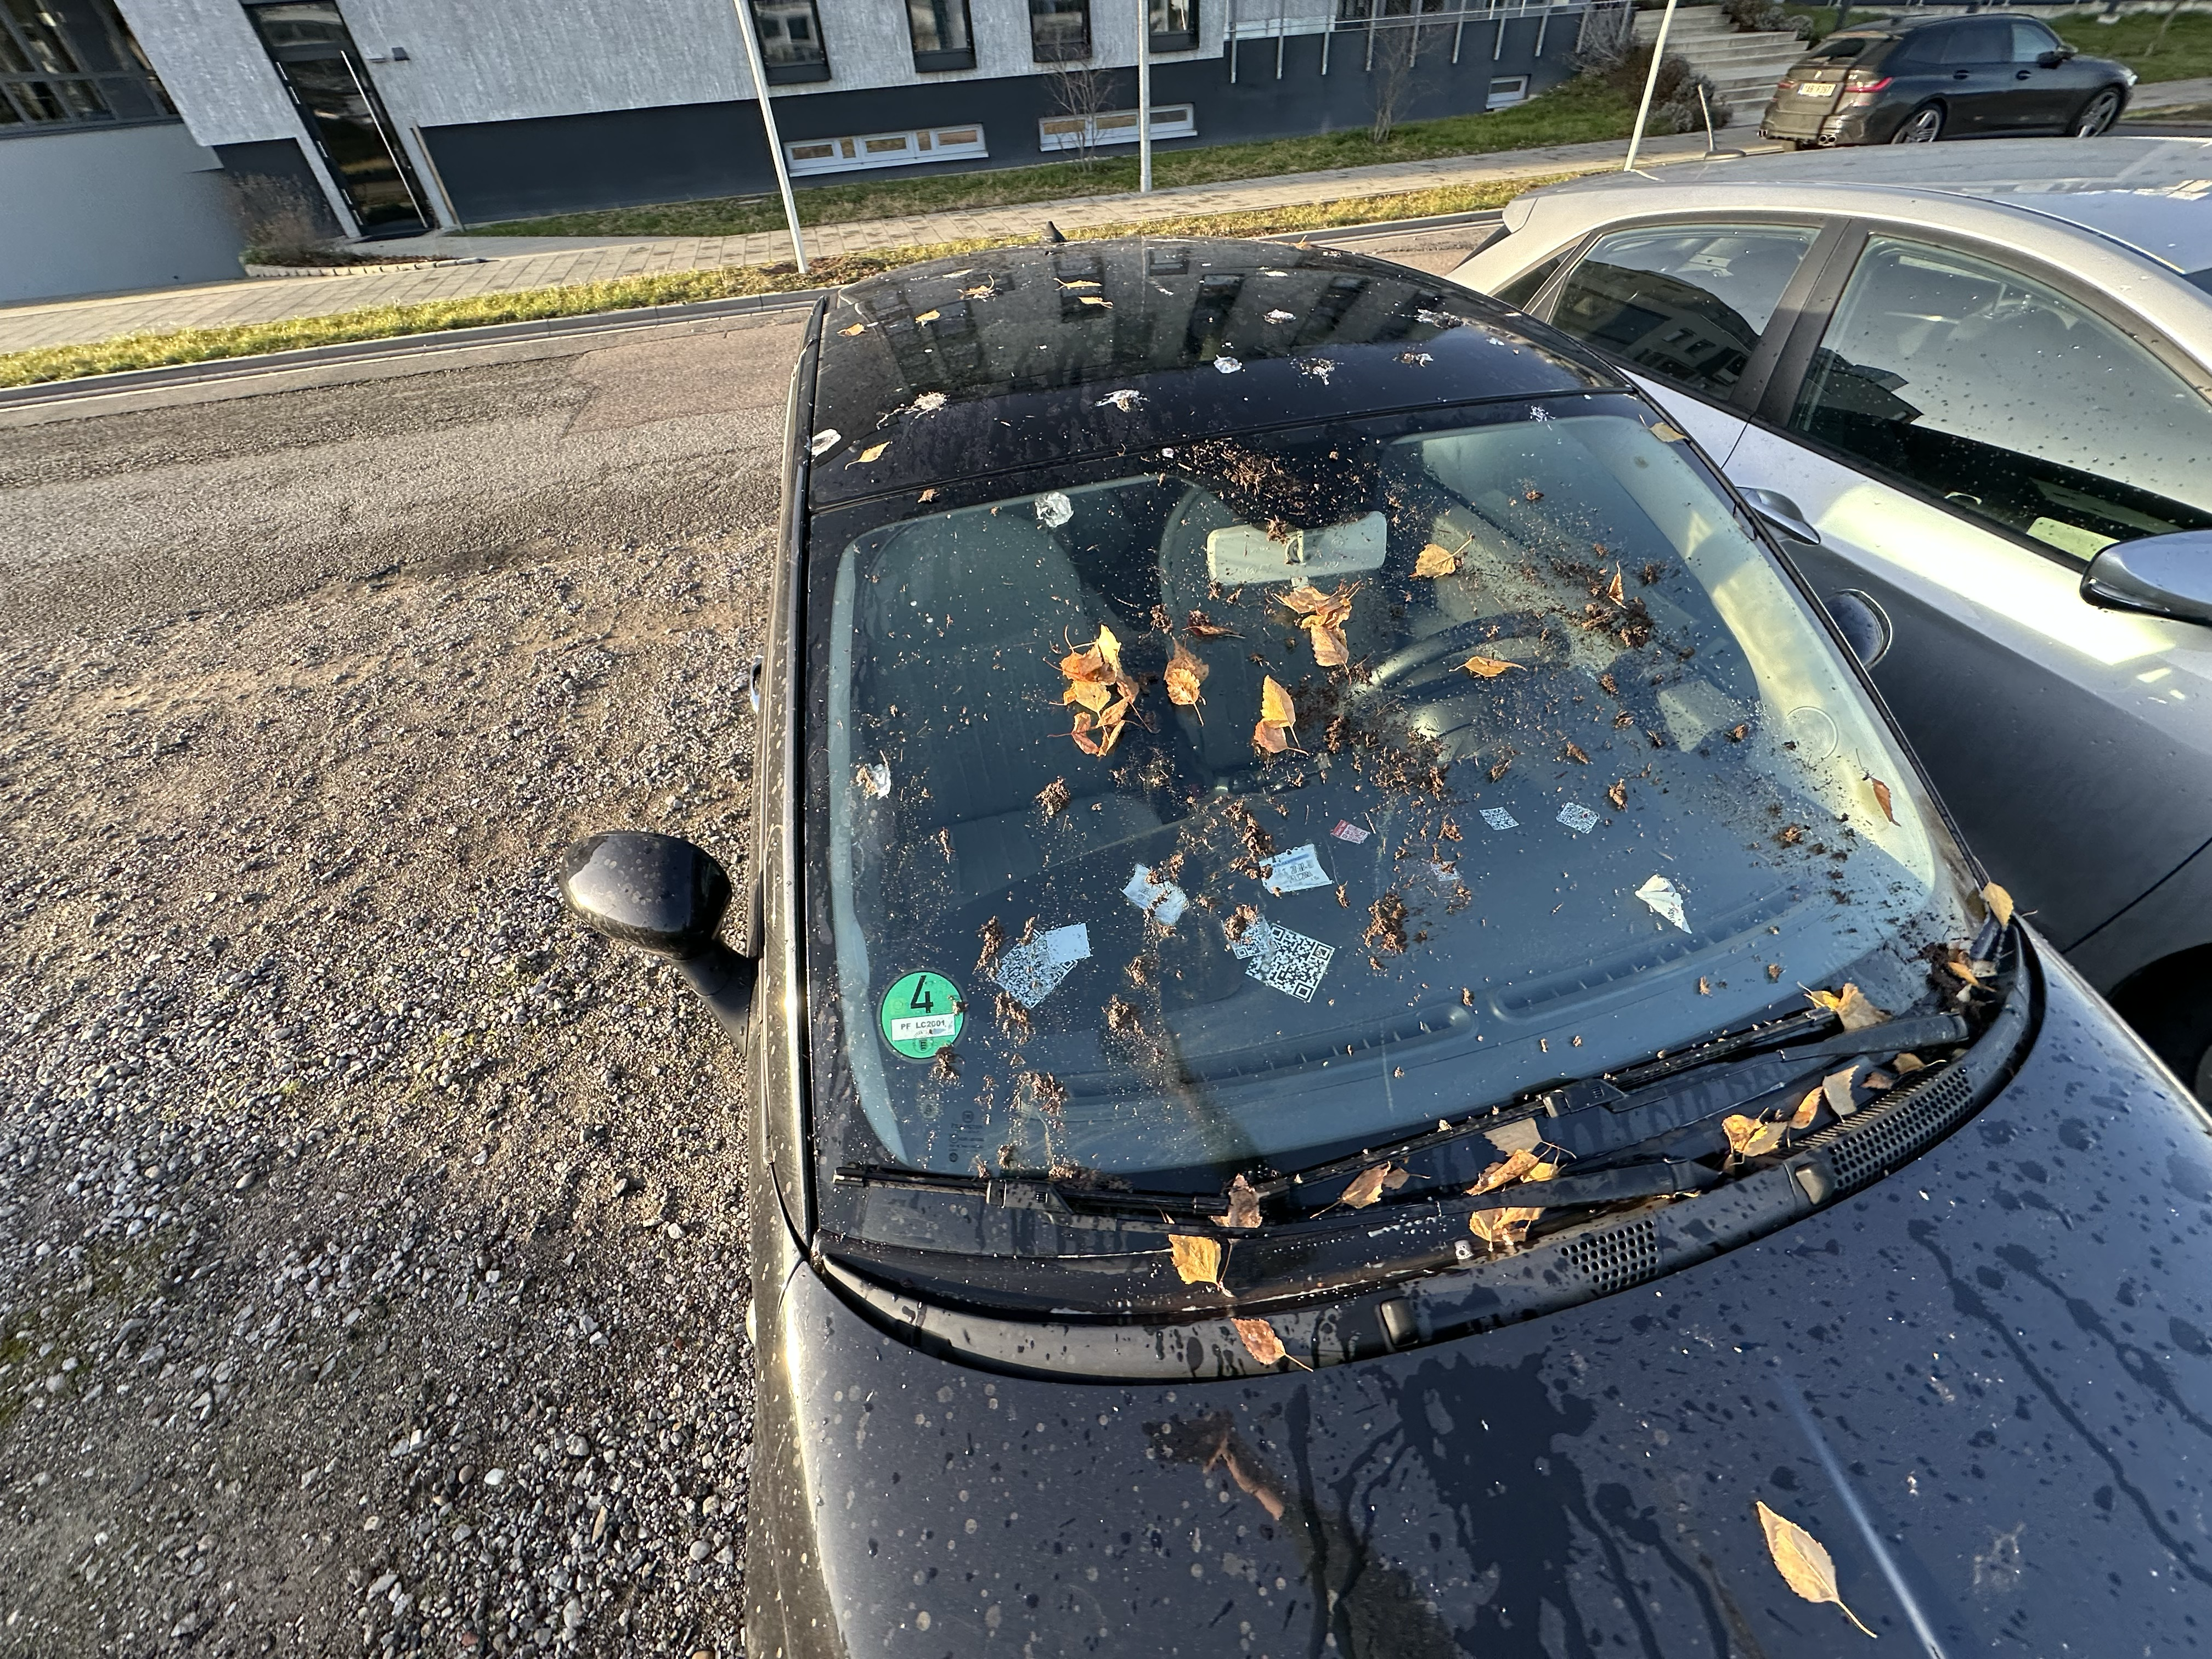
\includegraphics[width=\linewidth]{Figures/png/example_fiat_dirty.png}
        \caption*{(a) Fiat 500: stark verschmutzt, u.\,a. Kies/Reflexionen}
    \end{minipage}
    \hfill
    \begin{minipage}[t]{0.49\linewidth}
        \centering
        % Pfad anpassen:
        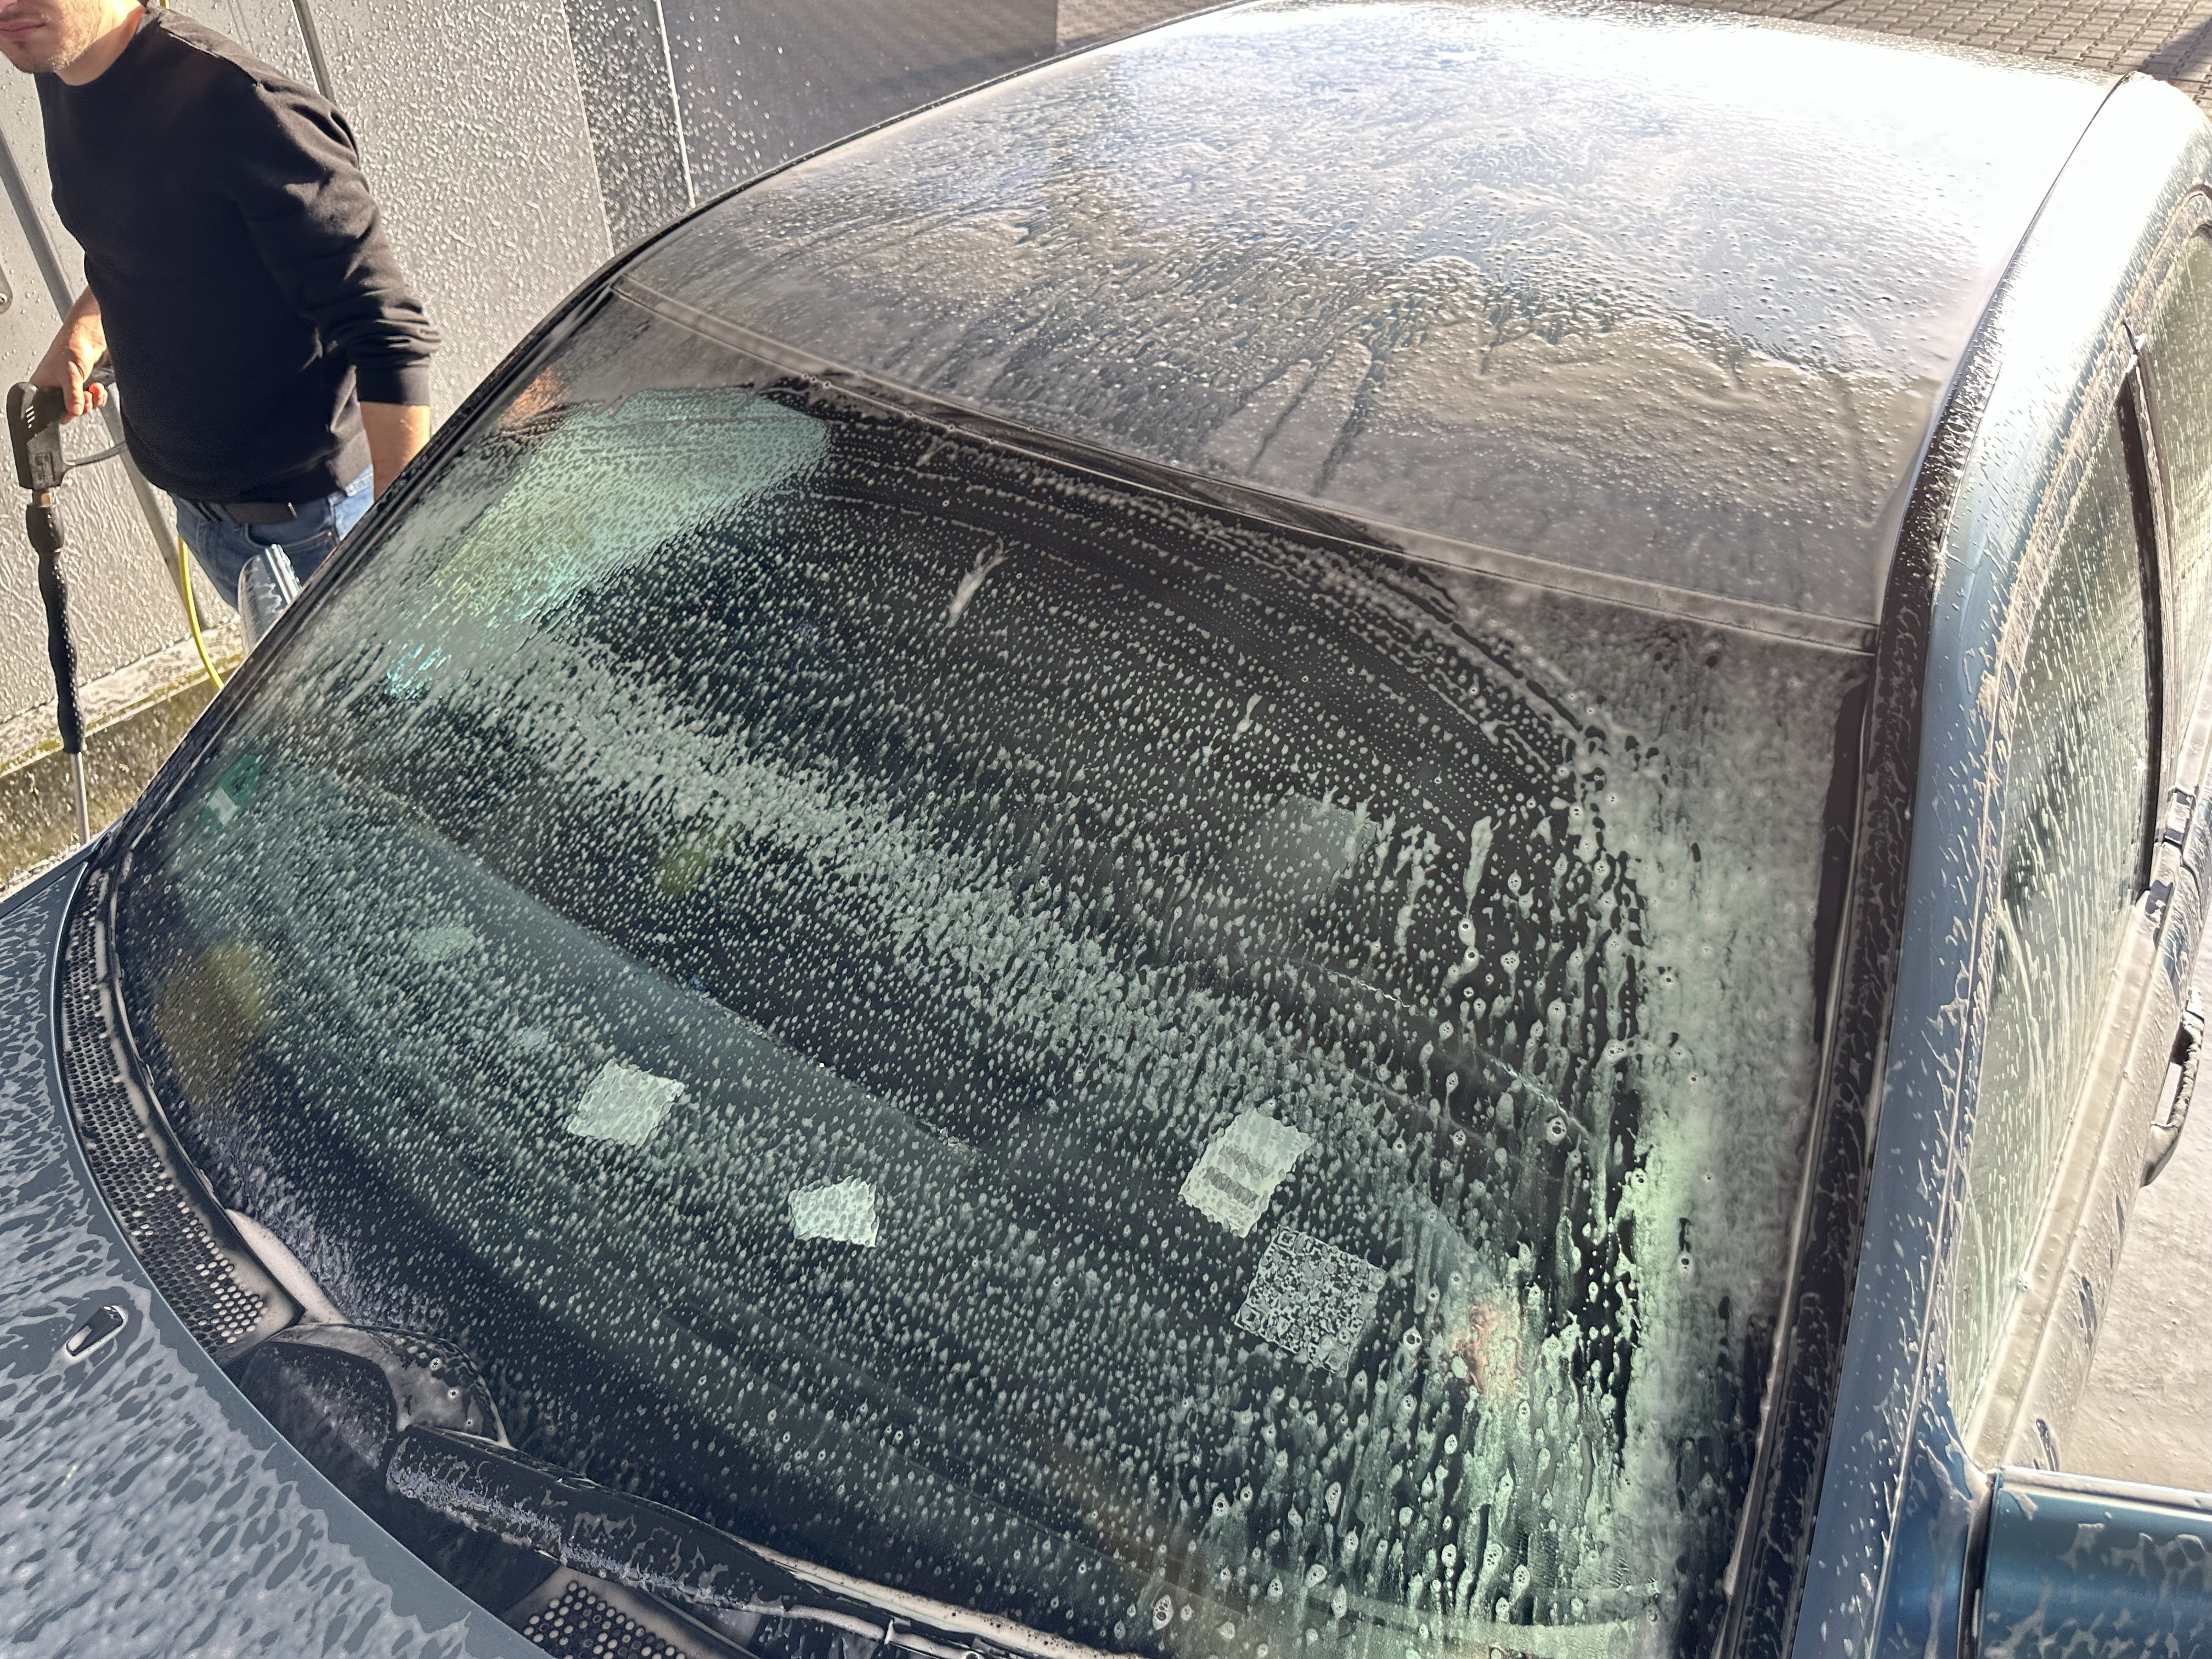
\includegraphics[width=\linewidth]{Figures/png/example_mercedes_foam.png}
        \caption*{(b) Mercedes W202: nasse/eingeschäumte Scheibe (Waschanlage)}
    \end{minipage}
    \caption{Beispielbilder aus den eigenen Aufnahmen: \ac{QR}-Codes hinter der Windschutzscheibe unter erschwerten Bedingungen.}
    \label{fig:dataset_examples}
\end{figure}

\subsection{Patch-Datensatz und Klassenverteilung}
\label{sec:patch_dataset}
Für das Training des \ac{CNN} wurde aus den hochauflösenden Bildern ein Patch-Datensatz aufgebaut. Hintergrund ist, dass der \ac{QR}-Code im Gesamtbild häufig nur einen kleinen Anteil einnimmt. Eine Patch-basierte Verarbeitung erlaubt es, relevante Bildbereiche in ausreichender Auflösung zu betrachten und dem \ac{CNN} eine konstante Eingabegröße bereitzustellen.

\begin{listNorm}
    \item \textbf{Patchgröße:} $265\,\times\,265$\,Pixel (konstante \ac{CNN}-Eingabe).
    \item \textbf{Manuelles Labeling:} ca. 26\,000 extrahierte Patches wurden manuell in \emph{\ac{QR}-Code} vs.~\emph{No \ac{QR}-Code} klassifiziert.
    \item \textbf{Augmentierung:} Rotation und horizontales Flippen der positiven \emph{\ac{QR}-Code}-Patches, um die positive Klasse zu erweitern und die Robustheit gegenüber Orientierungsvariationen zu erhöhen.
    \item \textbf{Klassenunwucht:} \emph{No \ac{QR}-Code} ist deutlich häufiger (insgesamt 49\,602 Patches nach Augmentierung) als \emph{\ac{QR}-Code}.
    \item \textbf{Positive Klasse:} rund 1\,500 \emph{\ac{QR}-Code}-Patches; nach Spiegelung ergeben sich 3\,066 \emph{\ac{QR}-Code}-Patches.
    \item \textbf{Balancierung:} Für das Training wird die negative Klasse pro Split zufällig auf die Größe der positiven Klasse heruntergesampelt (50/50).
\end{listNorm}

Die Aufteilung in Trainings-, Validierungs- und Testdaten erfolgt nicht durch Kopieren in neue Ordner, sondern wird als JSON-Datei gespeichert. Dabei werden Patches nach Quellbild gruppiert, um Datenleckage zu vermeiden (ein Quellbild erscheint nicht in mehreren Splits).

\newpage
\section{Bildvorverarbeitung}
\label{sec:bildvorverarbeitung}

\subsection{Motivation: Regionen statt Full-Image-Klassifikation}
\label{sec:roi_motivation}
Im Rahmen der Vorlesung wurde das Prinzip von Two-Stage-Detektoren vorgestellt, bei denen zunächst Kandidatenregionen (\emph{\ac{RoI}-Proposals}) bestimmt und anschließend klassifiziert werden. Dieser Gedanke wurde in diesem Projekt bewusst aufgegriffen, um erstmals eine Pipeline zu realisieren, die nicht nur das Gesamtbild klassifiziert, sondern gezielt Regionen extrahiert und einem \ac{CNN} zuführt. \cite{friedrich2025_cv,girshick2015_fast_rcnn}

Für das vorliegende Szenario ist dieser Ansatz insbesondere deshalb sinnvoll, weil \ac{QR}-Codes im Bild oft klein sind und bei starkem Downscaling des Gesamtbilds an Struktur verlieren. Durch die Patch-Erzeugung können relevante Bildbereiche in höherer Auflösung betrachtet werden und Störeinflüsse (Reflexionen, Schmutz, weitere Objekte) in Form negativer Beispiele explizit in den Trainingsprozess einfließen.

\subsection{ROI-Scoring: Heuristische Kandidatensuche}
\label{sec:roi_scoring}
Zur automatischen Erzeugung plausibler Kandidatenbereiche wird zunächst eine Score-Map berechnet, die pro Pixel eine \ac{QR}-ähnliche Strukturstärke repräsentiert. Die Score-Map kombiniert mehrere klassische Bildmerkmale, die für gedruckte \ac{QR}-Codes typisch sind:

\begin{listNorm}
    \item \textbf{Kanten (Canny):} \ac{QR}-Codes besitzen viele harte Schwarz/Weiß-Übergänge. Eine Kantenkarte liefert daher ein robustes Signal für strukturierte, kontrastreiche Bereiche.
    \item \textbf{Ecken (Harris):} Finder-Pattern und Modulraster erzeugen viele stabile Eckpunkte. Harris-Ecken sind daher ein geeignetes Indiz für \ac{QR}-ähnliche Regionen.
    \item \textbf{Gradientenstärke (Sobel-Magnitude):} Ergänzt Kanten/Ecken um ein kontinuierliches Kontrastmaß und stabilisiert die Bewertung bei wechselnden Schwellenwerten.
    \item \textbf{Anisotropie (Strukturtensor-basiert):} \ac{QR}-Codes enthalten regelmäßig ausgerichtete Kantenstrukturen. Ein Anisotropie-Maß hilft, solche Muster gegenüber flächigem Rauschen hervorzuheben.
\end{listNorm}

Die Merkmale werden gewichtet aufsummiert und anschließend normalisiert. In frühen Tests zeigte sich, dass Hintergrundobjekte mit starken Kanten/Ecken (z.\,B. Schlüssel oder Innenraumdetails) die Score-Map dominieren können. Die Gewichtung und Schwellwerte sind daher entscheidend, um die Spezifität für \ac{QR}-Codes zu erhöhen.
\newpage
\subsection{Multi-Scale Window Search und Redundanzreduktion}
\label{sec:roi_search}
Aus der Score-Map werden Kandidatenfenster über mehrere Skalen bestimmt:
\begin{listNorm}
    \item \textbf{Multi-Scale:} Abdeckung unterschiedlicher \ac{QR}-Code-Größen (Abstand/Zoom) durch mehrere Fenstergrößen.
    \item \textbf{Coarse-to-Fine:} Zunächst grobe Abtastung (großer Stride), anschließend lokale Verfeinerung um die besten Kandidaten (kleiner Stride).
    \item \textbf{Filterung über \ac{IoU}:} Stark überlappende Fenster werden unterdrückt, um redundante Patches zu vermeiden (Non-Maximum Suppression).
\end{listNorm}

Anschließend werden um die besten Kandidatenzentren quadratische Patches extrahiert und gespeichert. Optional werden zusätzlich gedrehte Varianten erzeugt, um geneigte Zettel und schräg platzierte \ac{QR}-Codes im Training abzudecken.

\subsection{Interaktives Parameter-Tuning (ROI-Tuner GUI)}
\label{sec:roi_gui}
Zur Parametrisierung der Score-Map und der Window-Suche wurde ein interaktives \ac{GUI} entwickelt. Dieses ermöglicht es, Gewichte und Schwellwerte live zu verändern und direkt zu beobachten, wie sich die Kandidatenfenster im Bild verhalten. Abbildung~\ref{fig:roi_tuner_gui} zeigt beispielhaft die Heatmap (links) sowie die Parametrierung über Regler (rechts). Die finalen Parameter werden als JSON-Konfiguration gespeichert und für die Batch-Extraktion verwendet.

\begin{figure}[H]
    \centering
    % Pfad anpassen:
    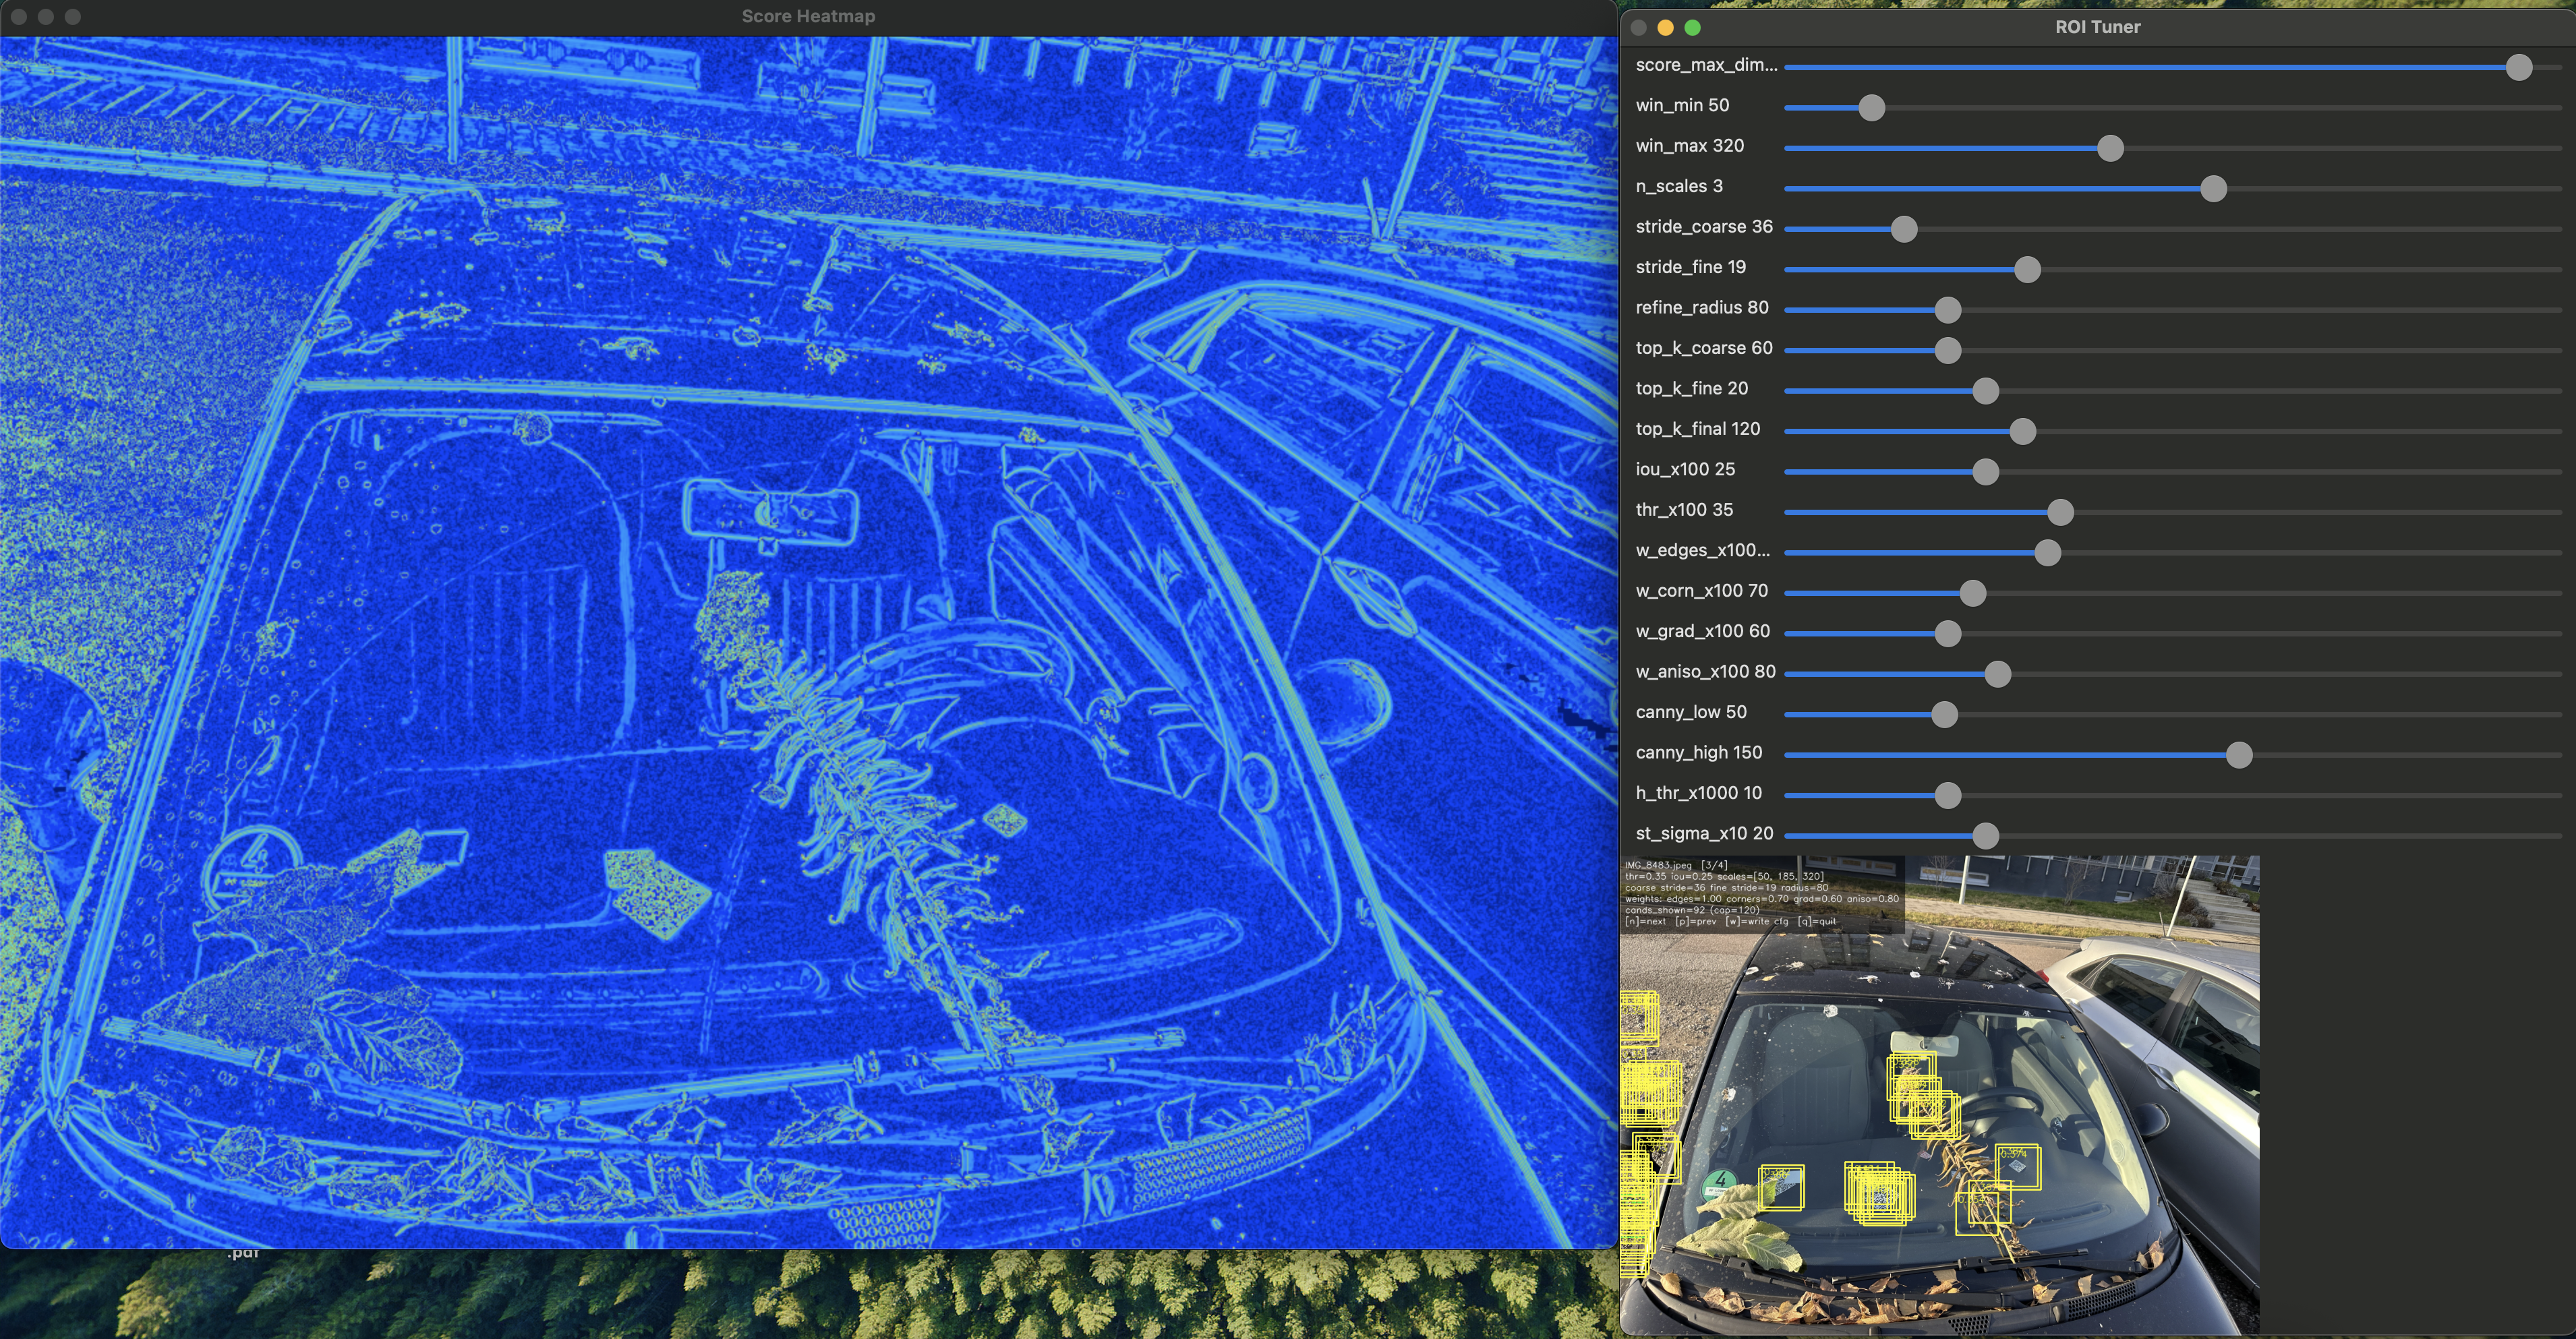
\includegraphics[width=\VarPicWidthD]{Figures/png/roi_tuner_gui.png}
    \caption{ROI-Tuner \ac{GUI}: links Score-Heatmap der kombinierten Merkmale, rechts Parameter-Regler sowie Vorschau der Kandidatenfenster im Originalbild.}
    \label{fig:roi_tuner_gui}
\end{figure}

Zusätzlich wurde ein Click-basiertes Auto-Tuning prototypisch erprobt, um Parameter automatisch zu optimieren. In der Praxis erwies sich dieser Ansatz als nicht ausreichend stabil, da die Optimierung häufig großflächig hohe Score-Werte erzeugte und dadurch die Kandidatenauswahl weniger spezifisch auf \ac{QR}-Codes reagierte. Die finale Parametrisierung wurde daher \ac{GUI}-gestützt manuell vorgenommen.


\section{Data Augmentation}
\label{sec:dataaugmentation}
Um die Robustheit gegenüber realen Variationen (Neigung, Spiegelungen, unterschiedliche Orientierung des Zettels) zu erhöhen, werden einfache geometrische Augmentierungen eingesetzt:

\begin{listNorm}
    \item \textbf{Rotation:} Beim Patch-Export werden optional zusätzlich gedrehte Patch-Varianten erzeugt (zur Abdeckung geneigter \ac{QR}-Codes).
    \item \textbf{Flip:} Positive \emph{QR-Code}-Patches werden horizontal gespiegelt, um die positive Klasse zu erweitern und das Modell gegen Orientierungsvariationen zu stabilisieren.
\end{listNorm}

Die Augmentierungen werden ausschließlich zur robusten \emph{Erkennung} (\emph{QR-Code vorhanden} vs. \emph{nicht vorhanden}) eingesetzt. Die spätere Lesbarkeitsprüfung erfolgt davon getrennt auf den detektierten \ac{QR}-Regionen.

\subsection{Erstellung der Trainings-, Validierungs- und Test-Splits}
\label{subsec:patch_splits}

Nach der Extraktion und manuellen Annotation der \ac{ROI}-Patches (Klassen \texttt{qr} und \texttt{no\_qr}) werden die Daten in Trainings-, Validierungs- und Testdaten aufgeteilt. Die Split-Erstellung erfolgt automatisiert und wird als JSON-Datei gespeichert, sodass keine Daten dupliziert oder in neue Ordnerstrukturen kopiert werden müssen. 

\subsubsection{Leakage-Vermeidung durch gruppierte Splits}
Da aus einem einzelnen Ursprungsbild typischerweise viele, teils stark überlappende Patches entstehen, wäre eine rein zufällige Patch-Aufteilung problematisch: Sehr ähnliche Bildausschnitte desselben Ursprungsbildes könnten in verschiedenen Splits landen und die Evaluierung dadurch künstlich verbessern.  
Um dies zu vermeiden, erfolgt die Aufteilung nicht auf Patch-Ebene, sondern auf \emph{Source}-Ebene. Alle Patches, die aus demselben Ursprungsbild stammen, werden gemeinsam genau einem Split zugeordnet.

\subsubsection{Split-Strategie und Reproduzierbarkeit}
Die Splits werden mit festen Anteilen (Train/Val/Test) erzeugt und über einen festen Zufallsseed (\texttt{seed=42}) deterministisch reproduzierbar gemacht. Die resultierenden Splits umfassen insgesamt 62 eindeutige Sources, verteilt auf 
\begin{listNorm}
    \item Training: 49 Sources,
    \item Validierung: 6 Sources und
    \item Test: 7 Sources
\end{listNorm}

\subsubsection{Balancierung der Klassenverteilung}
Die Rohdaten sind stark unausgeglichen (deutlich mehr \texttt{no\_qr}-Patches als \texttt{qr}-Patches). Für ein stabiles Training des binären Klassifikators wird daher \emph{pro Split} eine 50/50-Verteilung hergestellt. Dazu wird innerhalb jedes Splits die Mehrheitsklasse (\texttt{no\_qr}) zufällig heruntergesampelt, bis die Anzahl der \texttt{no\_qr}-Patches der Anzahl der \texttt{qr}-Patches entspricht (siehe Tabelle~\ref{tab:patch_splits}). 

\subsubsection{Ablageformat (JSON)}
Die fertigen Splits werden als JSON gespeichert. Jede Sample-Instanz enthält den relativen Dateipfad, das Label (\texttt{y=0} für \texttt{no\_qr}, \texttt{y=1} für \texttt{qr}) sowie die zugehörige Source-ID. Dieses Format wird in den Trainingsskripten direkt eingelesen und erlaubt eine saubere, versionierbare Datenaufteilung. 

\begin{table}[htbp]
    \centering
    \caption{Patch-Splits nach Source-gruppierter Aufteilung (keine Source-Überlappung) und 50/50-Balancierung pro Split.}
    \begin{tabular}{lrrrr}
        \hline
        \textbf{Split} & \textbf{Gesamt} & \textbf{no\_qr} & \textbf{qr} & \textbf{Unique Sources} \\
        \hline
        Training     & 4776 & 2388 & 2388 & 49 \\
        Validierung  & 496  & 248  & 248  & 6  \\
        Test         & 864  & 432  & 432  & 7  \\
        \hline
    \end{tabular}
    \label{tab:patch_splits}
\end{table}


	\chapter{CNN-Eigenentwicklung}
\label{ch:cnn_eigen}

\section{Netzarchitektur}
\label{sec:architektur_eigen}
% Anforderung: Aufbau des Netzes (Schichten, Neuronen, Filtergrößen)

\section{Hyperparameter und Optimierung}
\label{sec:hyperparameter_eigen}
% Anforderung: Überblick über verwendete und veränderte Hyperparameter (Epochen, Batchsize, LR, Optimizer, Loss, etc.)

\section{Ergebnisse}
\label{sec:ergebnisse_eigen}
% Anforderung: Kennzahlen, Konvergenz-Lossfunktionen, Accuracy für optimierte Parameter
	\chapter{Transfer Learning}
\label{ch:transfer}

\section{Untersuchte Modelle}
\label{sec:modelle_transfer}
% Anforderung: 3 verschiedene Modelle testen

\section{Vergleich und Ergebnisse}
\label{sec:ergebnisse_transfer}
% Anforderung: Geänderte Hyperparameter und Kennzahlen für alle 3 Netze
	\chapter{QR-Code Lokalisierung und Analyse}
\label{ch:qr_localization}

Dieses Kapitel beschreibt die praktische Pipeline zur \textbf{Lokalisierung} eines QR-Codes im Gesamtbild sowie die anschließende \textbf{Lesbarkeitsprüfung}. Anders als im reinen Patch-Training (Kapitel~\ref{ch:cnn_eigen} und Transfer Learning) wird hier die gesamte Windschutzscheiben-Szene verarbeitet und in mehreren Stufen zu einer finalen QR-Region verdichtet.

\section{Verfahren zur Positionsbestimmung}
\label{sec:pos_bestimmung}

\subsection{Motivation und GUI-Unterstützung}
\label{subsec:gui_motivation}

Zur Entwicklung und Bewertung der Lokalisierungs-Pipeline wurde ein eigenes GUI-Tool implementiert. Ziel war, die komplette Kette aus \ac{ROI}-Vorschlägen $\rightarrow$ CNN-Klassifikation $\rightarrow$ Merging $\rightarrow$ QR-Decoding interaktiv zu testen, zu debuggen und schnell gegeneinander zu vergleichen. Im GUI können dazu:
\begin{itemize}
    \item beliebige Trainings-Runs (inkl. Transfer-Modelle und From-Scratch CNN) geladen werden,
    \item Schwellwerte für die Patch-Klassifikation und das Merging live angepasst werden,
    \item die Zwischenergebnisse in fünf Ansichten visualisiert werden (Original, ROIs, Predictions, Merged-ROIs, Readability),
    \item und die Lesbarkeitsprüfung mit mehreren QR-Readern parallel ausgeführt werden.
\end{itemize}
Das war besonders hilfreich, um typische Fehlerbilder (z.\,B. harte Negativbeispiele durch starke Kanten, Spiegelungen oder Hintergrundobjekte) visuell zu verstehen und Parameter so zu wählen, dass die QR-Region im realistischen Szenario stabil wiedergefunden wird. :contentReference[oaicite:1]{index=1}

\subsection{Stufe 1: ROI-Vorschläge (Region Proposals)}
\label{subsec:stage1_rois}

Die Positionsbestimmung startet mit der Erzeugung von Kandidatenregionen (\acp{ROI}) im Vollbild. Dazu werden aus dem Bild zunächst \textbf{ROI-Zentren} vorgeschlagen (im GUI über eine gespeicherte ROI-Konfiguration aus dem ROI-Tuner), und um jedes Zentrum wird ein Patch fester Größe ausgeschnitten. Diese Patch-Größe entspricht der für das Training verwendeten Patch-Größe (typisch $265 \times 265$ Pixel), damit das CNN auf exakt den Daten arbeitet, auf denen es gelernt hat. Zusätzlich existiert ein Cap (z.\,B. 200 Patches pro Bild), um die Laufzeit zu begrenzen. :contentReference[oaicite:2]{index=2}

\subsection{Stufe 2: Patch-Klassifikation (QR vs. No-QR)}
\label{subsec:stage2_cnn}

Jeder vorgeschlagene Patch wird anschließend durch das gewählte Modell klassifiziert. Das GUI unterstützt dabei sowohl:
\begin{itemize}
    \item \textbf{Scratch-Modelle} (eigenes CNN, Input typischerweise $265\times265$),
    \item als auch \textbf{Transfer-Modelle} (z.\,B. EfficientNet-B0 / MobileNetV3-Large / ResNet18, Input typischerweise $224\times224$ mit ImageNet-Normalisierung).
\end{itemize}
Die Ausgabe wird als Wahrscheinlichkeit $p(\text{QR})$ interpretiert (Sigmoid/Softmax je nach Output-Shape). Anschließend wird per Schwellwert $\texttt{thr}$ entschieden, ob ein Patch als QR-positiv gilt. :contentReference[oaicite:3]{index=3}

\textbf{Empirische Einstellung (EfficientNet-B0):} Für EfficientNet-B0 hat sich im Projekt ein hoher Klassifikationsschwellwert von
\[
\texttt{thr}=0.95
\]
als sehr robust erwiesen. Die Intuition dahinter: Im Vollbild entstehen viele \ac{ROI}-Vorschläge auf starken Kantenstrukturen (A-Säule, Wischer, Dachkante, Spiegelungen, Hintergrund). Ein hoher Schwellenwert reduziert diese False Positives deutlich und lässt bevorzugt nur sehr sichere QR-Kandidaten übrig, die anschließend gemerged werden.

\subsection{Stufe 3: Merging zu einer finalen QR-Region}
\label{subsec:stage3_merge}

Da ein echter QR-Code typischerweise \textbf{mehrere} positive Patches erzeugt (überlappende Treffer um die gleiche Region), werden alle QR-positiven Patch-Boxen anschließend zu zusammenhängenden Kandidatenregionen zusammengefasst.

Das Merging erfolgt als \textbf{IoU-basiertes Clustering}: Zwei Boxen gehören zur gleichen Gruppe, wenn ihre Intersection-over-Union (IoU) mindestens dem Merging-Schwellwert entspricht. Daraus werden Connected Components gebildet; pro Cluster entsteht eine \textbf{Union-Box} als finaler Kandidat. Als Score des Kandidaten wird der maximale Patch-Score im Cluster verwendet. :contentReference[oaicite:4]{index=4}

\textbf{Empirische Einstellung (EfficientNet-B0):} Für das Merging hat sich
\[
\texttt{merge\_iou}=0.30
\]
als praktikabel erwiesen. Die Intuition: QR-Treffer liegen oft nur teilweise überlappend (je nach Patch-Zentrum), und ein zu hoher IoU-Schwellwert würde Treffergruppen unnötig aufsplitten. Mit $0.30$ werden benachbarte, klar zusammengehörige Treffer stabil zu einer Region verdichtet.

\subsection{Visualisierung der fünf Ansichten}
\label{subsec:views}

Abbildung~\ref{fig:gui_views} zeigt die fünf GUI-Ansichten anhand desselben Beispiels:
\begin{itemize}
    \item \textbf{(1) Original:} unverändertes Vollbild,
    \item \textbf{(2) ROIs (gelb):} alle vorgeschlagenen Patch-Regionen,
    \item \textbf{(3) Predictions (rot/grün):} Patch-Boxen nach Klassifikation (grün: $p\ge\texttt{thr}$),
    \item \textbf{(4) Merged QR crops (cyan):} gemergte Kandidatenregion(en) aus positiven Patches,
    \item \textbf{(5) Readability (rot/grün) + Liste:} finale Region(en) nach Decoding-Prüfung (grün = lesbar).
\end{itemize}

\begin{figure}[htbp]
    \centering

    \begin{minipage}{0.49\linewidth}
        \centering
        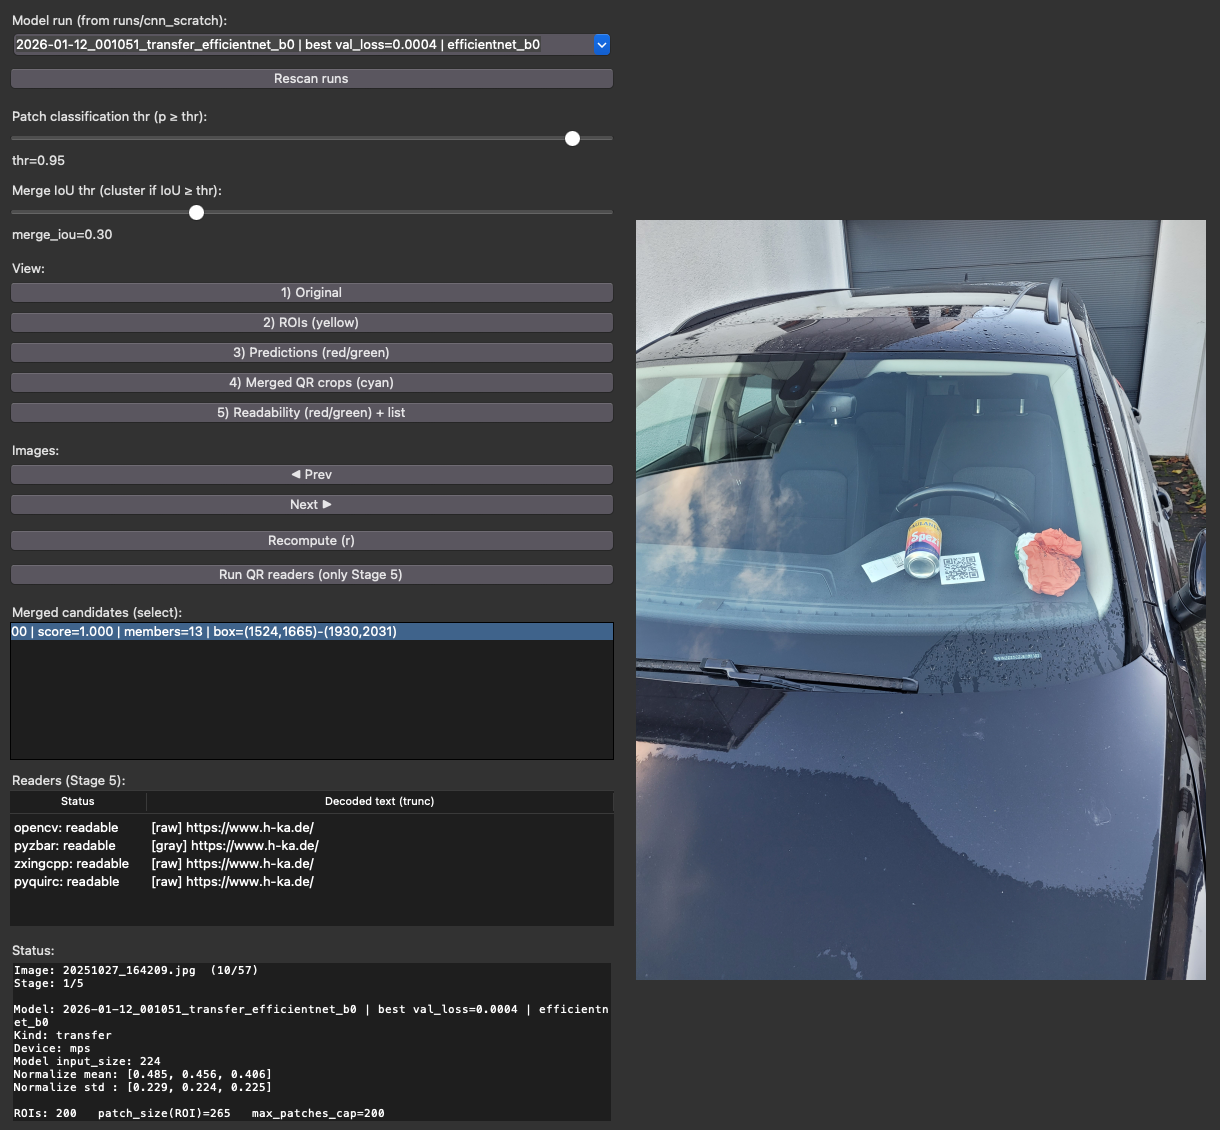
\includegraphics[width=\linewidth]{Figures/png/gui_view1_original.png}
        \caption*{(1) Original}
    \end{minipage}\hfill
    \begin{minipage}{0.49\linewidth}
        \centering
        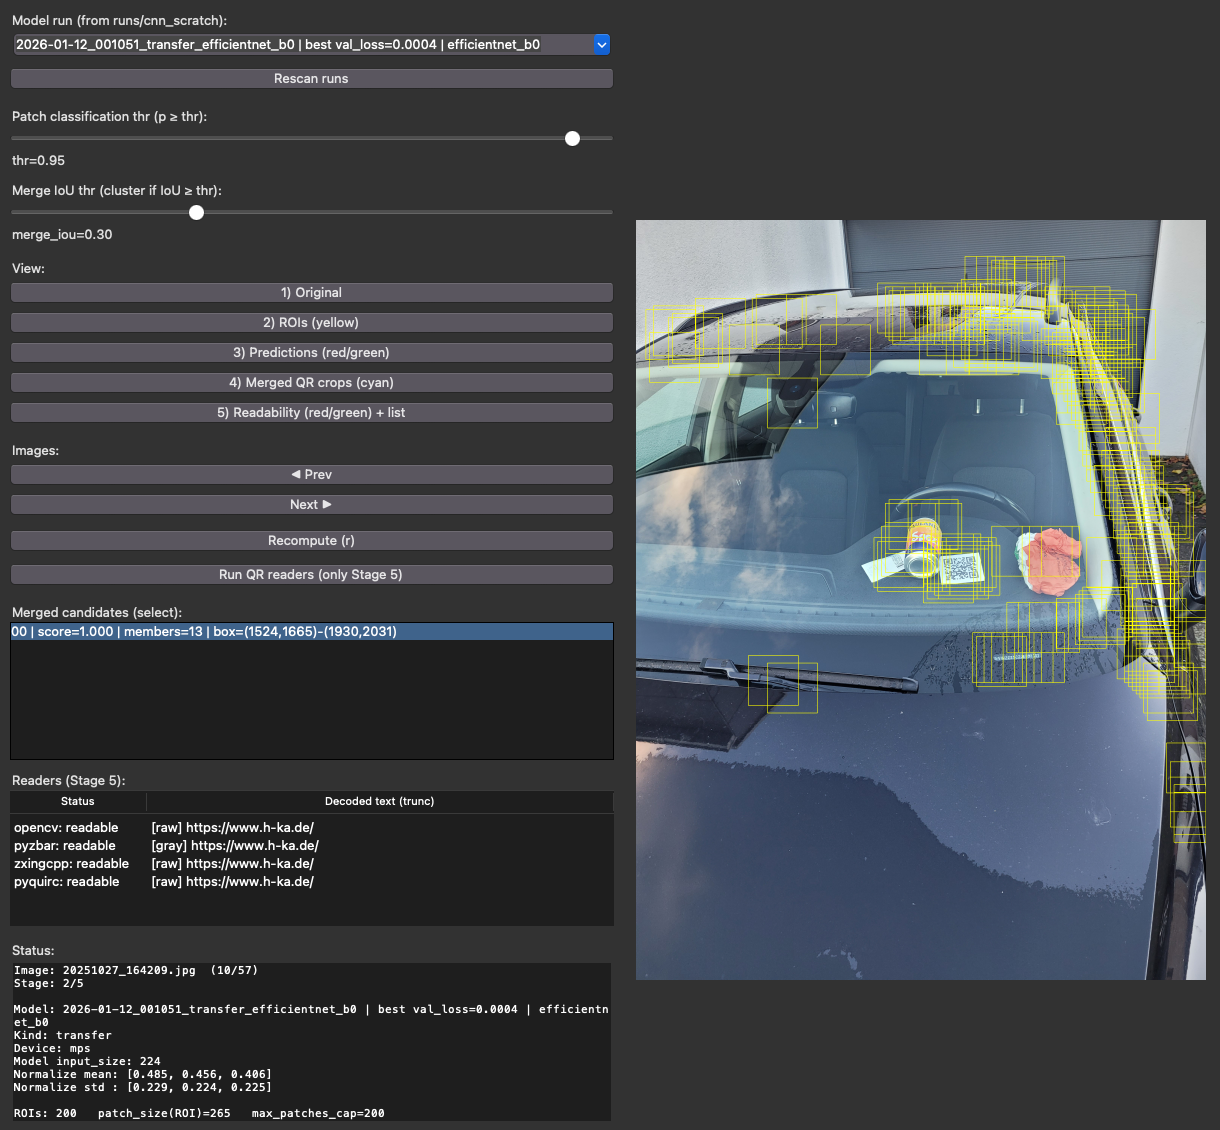
\includegraphics[width=\linewidth]{Figures/png/gui_view2_rois.png}
        \caption*{(2) ROIs (gelb)}
    \end{minipage}

    \vspace{0.6em}

    \begin{minipage}{0.49\linewidth}
        \centering
        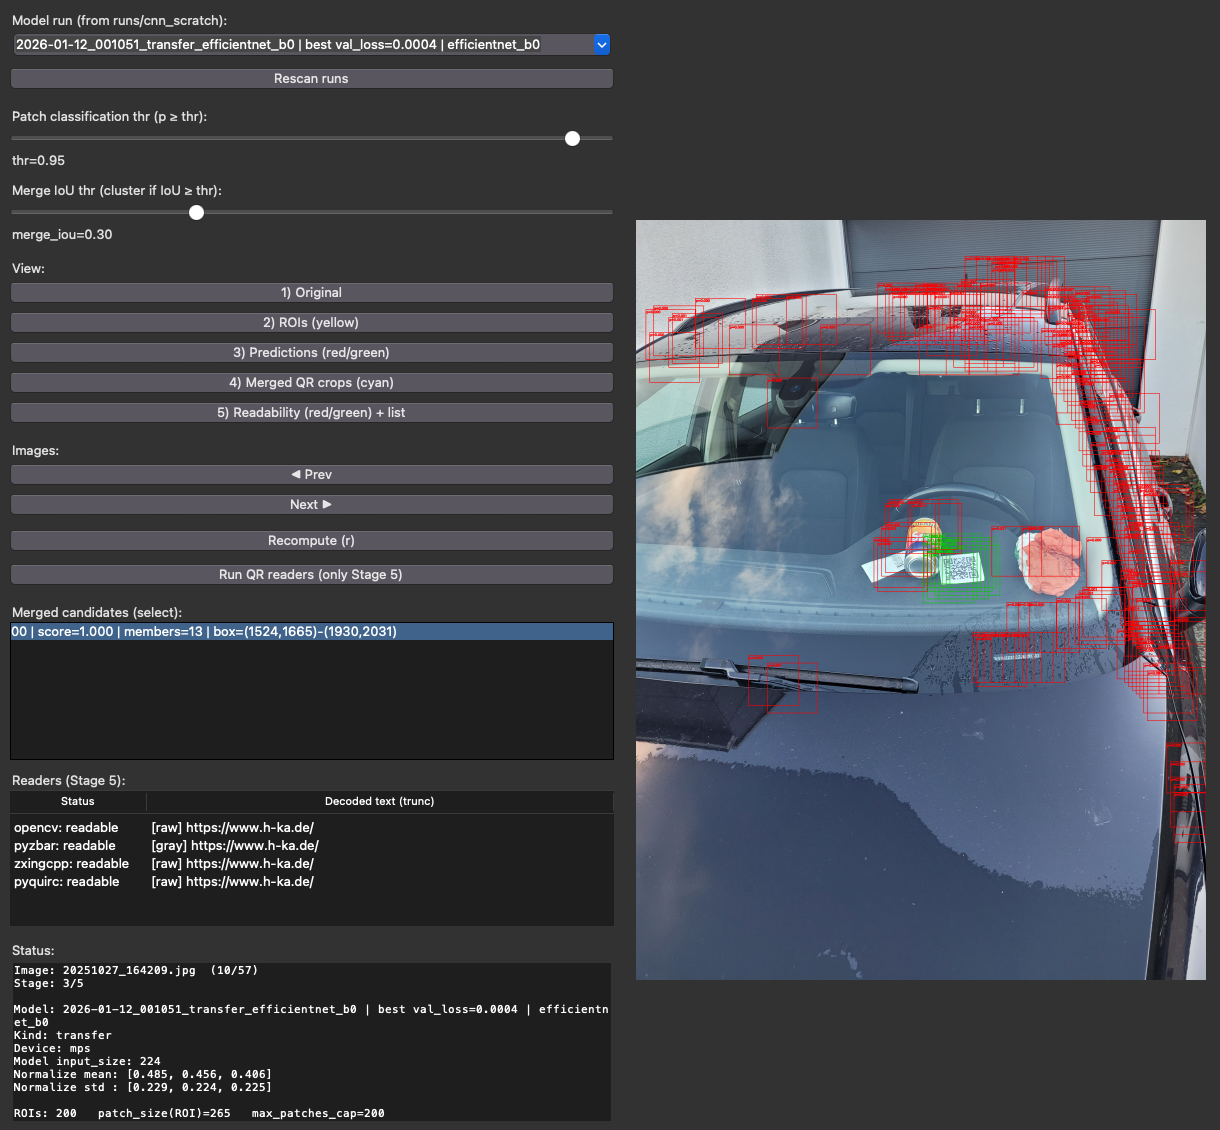
\includegraphics[width=\linewidth]{Figures/png/gui_view3_predictions.png}
        \caption*{(3) Predictions (rot/grün)}
    \end{minipage}\hfill
    \begin{minipage}{0.49\linewidth}
        \centering
        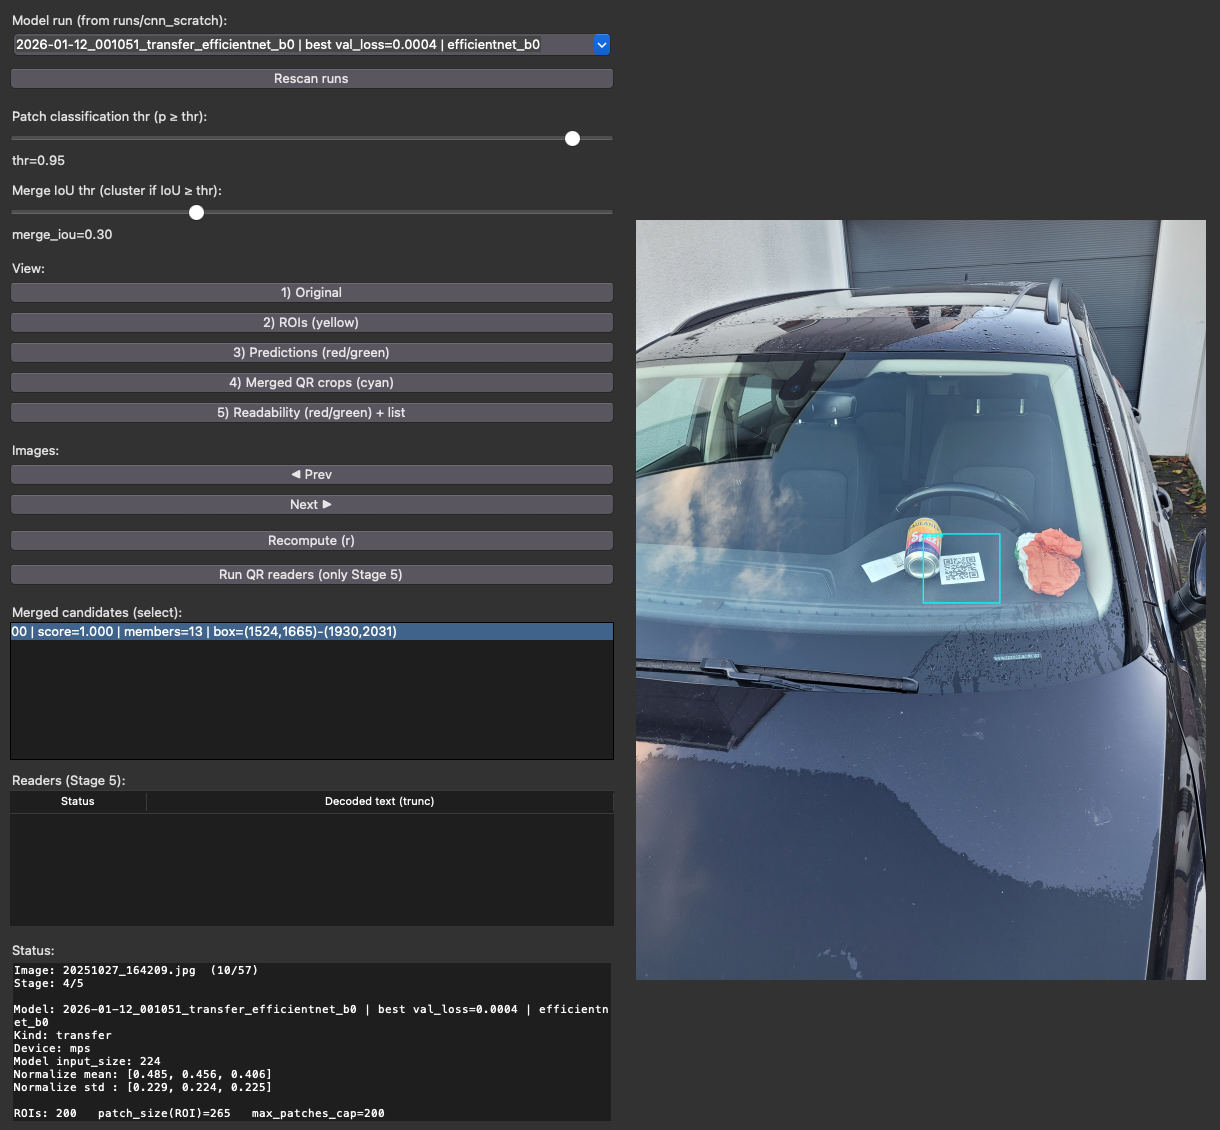
\includegraphics[width=\linewidth]{Figures/png/gui_view4_merged.png}
        \caption*{(4) Merged QR crops (cyan)}
    \end{minipage}

    \vspace{0.6em}

    \begin{minipage}{0.70\linewidth}
        \centering
        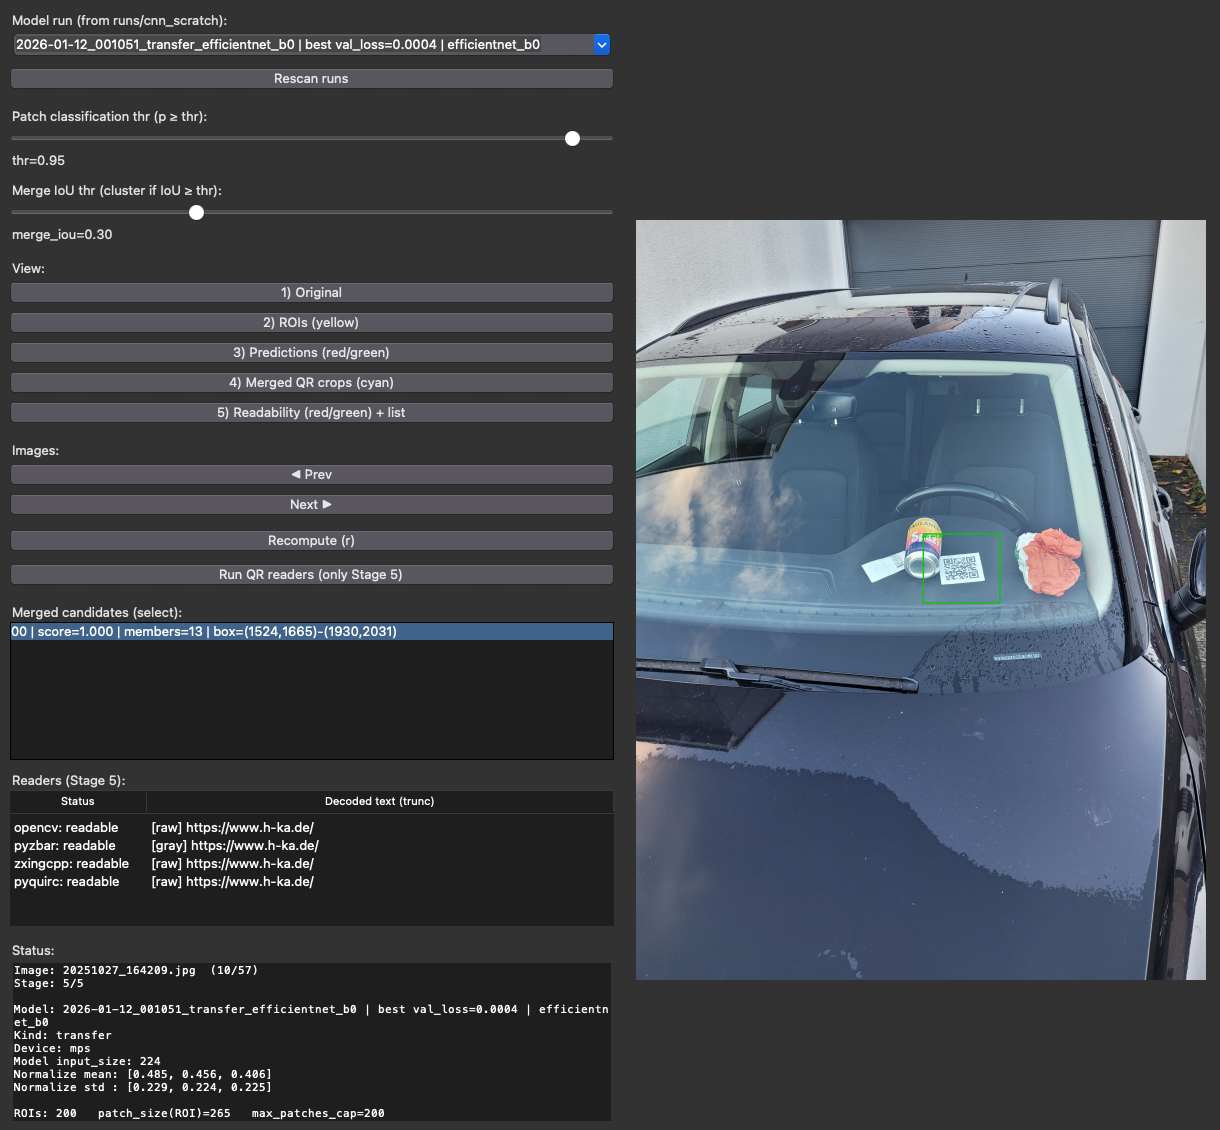
\includegraphics[width=\linewidth]{Figures/png/gui_view5_readability.png}
        \caption*{(5) Readability (rot/grün) + Reader-Liste}
    \end{minipage}

    \caption{Fünf Ansichten des Prediction-GUIs zur QR-Code-Lokalisierung und Lesbarkeitsprüfung (gleiches Bild, gleiche Modelleinstellungen).}
    \label{fig:gui_views}
\end{figure}


\section{Lesbarkeitsprüfung}
\label{sec:lesbarkeit}

\subsection{Motivation: Decoder sind inkonsistent}
\label{subsec:decoder_problem}

Nach dem Merging liegt pro Kandidat eine Box vor, die \glqq wahrscheinlich\grqq{} einen QR-Code enthält. Für die tatsächliche Nutzbarkeit ist jedoch entscheidend, ob der QR-Code auch \textbf{dekodierbar} ist. In der Praxis zeigte sich, dass einzelne QR-Decoder auf schwierigen Bildern (Reflexion, Nässe, Schaum, Bewegungsunschärfe, Kompressionsartefakte, Teilabdeckung) teils inkonsistent reagieren: Ein Decoder kann in einem Bild erfolgreich sein, während er im nächsten Bild trotz ähnlicher Situation scheitert.

Aus diesem Grund wurde eine \textbf{Multi-Reader-Strategie} implementiert: Mehrere Decoder laufen parallel, und sobald mindestens ein Decoder den QR-Code lesen kann, wird die Region als \textbf{lesbar} markiert (grüner Rahmen). Damit wird die Lesbarkeitsentscheidung deutlich stabiler als mit einem einzelnen Reader. :contentReference[oaicite:5]{index=5}

\subsection{Reader-Kaskade und Vorverarbeitungsvarianten}
\label{subsec:decoder_pipeline}

Im GUI werden folgende Reader genutzt (sofern installiert/verfügbar):
\begin{itemize}
    \item OpenCV \texttt{QRCodeDetector},
    \item \texttt{pyzbar},
    \item \texttt{zxingcpp},
    \item \texttt{pyquirc} (quirc).
\end{itemize}
Jeder Reader erhält nicht nur das rohe Crop, sondern mehrere einfache Vorverarbeitungsvarianten, um schwierige Fälle abzufangen:
\begin{itemize}
    \item \textbf{raw}: unverändertes Crop,
    \item \textbf{gray}: Graustufenvariante,
    \item \textbf{upscaled}: Vergrößerung kleiner Crops (Interpolation), falls die Region sehr klein ist,
    \item \textbf{adaptive threshold}: binarisierte Variante, die häufig bei Reflexionen oder ungleichmäßiger Beleuchtung hilft.
\end{itemize}
Der Reader versucht die Varianten der Reihe nach; sobald ein gültiger Text extrahiert wurde, gilt dieser Reader als erfolgreich. Die Ergebnisse werden im GUI als Liste angezeigt (Readername, Status, gekürzter Text und verwendete Variante). :contentReference[oaicite:6]{index=6}

\subsection{Kriterium: wann ist ein QR-Code lesbar?}
\label{subsec:lesbar_kriterium}

Ein gemergter Kandidat wird als \textbf{lesbar} klassifiziert, wenn mindestens einer der Reader einen nicht-leeren Decodetext liefert:
\[
\texttt{READABLE} \Leftrightarrow \exists\, r \in \{\text{Reader}\}:\ r(\text{Crop})\ \text{liefert Text}
\]
In diesem Fall wird die Kandidatenregion im Bild \textbf{grün} markiert; andernfalls \textbf{rot}. In der Praxis ergab sich, dass bestimmte Reader (z.\,B. \texttt{pyquirc} oder \texttt{zxingcpp}) in vielen Fällen robuster wirkten als OpenCV – jedoch nicht konstant in jedem Bild. Genau deshalb ist die Mehrfachausführung entscheidend: Sie erhöht die Wahrscheinlichkeit, dass zumindest ein Reader unter den jeweiligen Bildstörungen erfolgreich ist.

\subsection{Zwischenfazit}
\label{subsec:lesbarkeit_fazit}

Die Kombination aus (i) konservativem Patch-Threshold (\texttt{thr=0.95}), (ii) IoU-basiertem Merging (\texttt{merge\_iou=0.30}) und (iii) Multi-Reader-Decoding stellt eine robuste, gut interpretierbare Pipeline dar. Sie verbindet die gelernten CNN-Entscheidungen (QR vs. No-QR auf Patches) mit einer praktischen Nutzbarkeitsprüfung (dekodierbarer QR-Code) und ermöglicht über das GUI schnelle, nachvollziehbare Tests auf beliebigen Bildern.

	\chapter{Zusammenfassung und Ausblick}
\label{ch:outlook}

\section{Zusammenfassung}
Ziel dieser Projektarbeit war die robuste Erkennung und Analyse von QR-Codes hinter einer Windschutzscheibe unter realistischen Störbedingungen (Verschmutzung, Nässe/Schaum, Reflexionen, wechselnde Beleuchtung und störende Hintergrundobjekte). Dafür wurde eine durchgängige Pipeline entwickelt, die sich in drei Kernbausteine gliedert:

\begin{itemize}
    \item \textbf{Patch-basierter Datensatzaufbau:} Aus hochauflösenden Szenenbildern wurden quadratische Patches fester Größe extrahiert und manuell gelabelt. Die Aufteilung der Daten erfolgte source-basiert, um Datenleckage durch stark ähnliche Patches aus demselben Ursprungsbild zu vermeiden.
    \item \textbf{CNN-Klassifikation (QR vs.\ No-QR):} Es wurde zunächst ein eigenes CNN trainiert und systematisch über Konfigurations-Overrides optimiert. Im zweiten Schritt wurde Transfer Learning mit verschiedenen Backbones untersucht, um die Generalisierung bei begrenzter Datenmenge zu erhöhen.
    \item \textbf{Lokalisierung und Lesbarkeitsprüfung im Vollbild:} Aus \acp{ROI} und Patch-Predictions wurden über ein IoU-basiertes Merging finale Kandidatenregionen gebildet. Anschließend wurde die Nutzbarkeit über mehrere QR-Decoder parallel geprüft. Ergänzend wurde eine Geometrie-Pipeline entwickelt, die aus der detektierten QR-Fläche eine Top-View erzeugt und daraus Rotationswinkel als Grundlage für eine Kamerapositionierungs-Empfehlung ableitet.
\end{itemize}

Ein wichtiger praktischer Erkenntnisgewinn war, dass die Güte der Evaluierung maßgeblich von der korrekten Split-Strategie abhängt: Patch-basierte Splits können die Leistung künstlich erhöhen, wenn ähnliche Ausschnitte desselben Ursprungsbildes in Training und Test landen. Nach Umstellung auf source-basierte Splits wurden die Ergebnisse deutlich realistischer und damit belastbarer.

\section{Ausblick}
Im Projekt wurde eine vollständige Pipeline bis zur Lesbarkeitsbewertung und Winkelabschätzung umgesetzt. Für eine weitere Steigerung von Robustheit und Übertragbarkeit bieten sich insbesondere folgende Schritte an:

\subsection{Mehr Daten und mehr \textit{Unique Sources}}
Der stärkste Hebel für Generalisierung ist eine größere und diversere Datengrundlage. Besonders vorteilhaft wären:
\begin{itemize}
    \item mehr Ursprungsbilder aus unterschiedlichen Fahrzeugen, Windschutzscheiben-Geometrien und Innenräumen,
    \item mehr Variabilität in Distanz, Perspektive und QR-Größe,
    \item gezielte Abdeckung schwieriger Szenarien (Schaumcluster, starke Spiegelungen, Teilabdeckung, Motion Blur).
\end{itemize}
Mehr \textit{unique sources} reduziert die Gefahr, dass Modelle ungewollt auf fahrzeugspezifische Muster oder wiederkehrende Hintergründe reagieren, statt auf QR-Strukturen.

\subsection{Training nur mit Graustufen}
QR-Codes sind strukturell (Kontrast/Geometrie) und nicht farblich definiert. Ein nächster Schritt wäre daher ein Training ausschließlich auf Graustufen-Patches:
\begin{itemize}
    \item potenziell stabileres Lernen durch Reduktion irrelevanter Farbvariationen (Reflexionsfarbe, Lack-/Innenraumfarben),
    \item geringerer Rechenaufwand und weniger Parameterbedarf im ersten Layer,
    \item klarer Fokus auf Kanten, Module und Finder-Pattern.
\end{itemize}
Optional könnte man RGB und Gray auch als zweigleisige Eingabe testen (Early Fusion), um zu prüfen, ob Farbe in einzelnen Sonderfällen trotzdem hilft.

\subsection{Von heuristischen ROIs zu lernbasierten Region Proposals}
Die aktuelle ROI-Erzeugung basiert auf klassischen Bildmerkmalen und Filtermethoden. Das ist transparent und schnell, aber prinzipbedingt empfindlich gegenüber starken Kanten in Nicht-QR-Objekten (z.\,B.\ Innenraumdetails oder harte Hintergrundstrukturen). Als nächster Evolutionsschritt wäre eine lernbasierte Proposal-Strategie naheliegend:
\begin{itemize}
    \item \textbf{Two-Stage-Detektor (z.\,B.\ Faster R-CNN):} Ein RPN (Region Proposal Network) erzeugt Kandidatenregionen datengetrieben, die anschließend klassifiziert und regressiert werden. Damit würde die ROI-Auswahl nicht mehr durch Heuristiken, sondern durch ein trainiertes Proposal-Netz erfolgen.
    \item \textbf{End-to-End-Detektion statt Patch-Kaskade:} Alternativ wäre auch ein One-Stage-Detektor (z.\,B.\ YOLO/SSD) denkbar, der direkt Bounding Boxes für QR-Codes vorhersagt.
\end{itemize}
Gerade bei kleinen Objekten und stark variierenden Hintergründen kann ein trainierter Proposal-Mechanismus die Anzahl irrelevanter Kandidaten reduzieren und die Lokalisierung stabilisieren.

\subsection{Gezielte Evaluierung und robustere Modellwahl}
Um die Aussagekraft weiter zu erhöhen, wären sinnvoll:
\begin{itemize}
    \item source-basierte Cross-Validation (mehrere Folds), um die Abhängigkeit von einem einzelnen Split zu reduzieren,
    \item eine systematische Fehleranalyse (False Positives/Negatives) mit Kategorien wie \glqq Reflexion\grqq, \glqq Schaum\grqq, \glqq sehr klein\grqq, \glqq Hintergrundkanten\grqq,
    \item ein \glqq hard-negative mining\grqq{} Ansatz, bei dem besonders irreführende Negativpatches gezielt nachgelabelt und nachtrainiert werden.
\end{itemize}

\subsection{Verbesserungen an der Decoding-Stufe}
Die Lesbarkeitsprüfung hat gezeigt, dass einzelne QR-Reader inkonsistent sein können und die Multi-Reader-Strategie daher praktisch relevant ist. Als Ausblick bieten sich an:
\begin{itemize}
    \item erweiterte Preprocessing-Varianten (z.\,B.\ Deblurring, stärkere Super-Resolution für kleine Crops),
    \item eine Qualitätsmetrik für die Top-View (Schärfe/Modulkontrast) zur Priorisierung der Kandidaten,
    \item zeitliche Stabilisierung bei Videostreams (Tracking über Frames, Majority Vote über mehrere Bilder).
\end{itemize}

\subsection{Deployment-nahe Aspekte}
Für ein reales System in einer Waschanlage wären zusätzlich folgende Punkte zu beachten:
\begin{itemize}
    \item Laufzeitoptimierung (Quantisierung, ggf.\ kleinere Backbones),
    \item robuste Kamerahardware (z.\,B.\ Polarisationsfilter zur Reduktion von Reflexionen),
    \item definierte Montagegeometrie und ggf.\ mehrere Kameras/Winkel zur Redundanz.
\end{itemize}

\bigskip
Insgesamt zeigt das Projekt, dass die Kombination aus patch-basierter Klassifikation, nachvollziehbarem Merging und einer robusten Lesbarkeitsprüfung bereits eine praxistaugliche Grundlage bildet. Die größten Potenziale für den nächsten Schritt liegen in mehr und diverseren Daten sowie in einer lernbasierten, end-to-end Lokalisierung (Region Proposals) anstelle rein heuristischer ROI-Filterung.


	\begin{appendix}
		\input{TeXFiles/110_Anhang}
	\end{appendix}
	
	\clearpage

	%% If you want to change the bibliography heading, you can do so by using the following line
	\renewcommand*{\refname}{Literaturverzeichnis}

	%\bibliographystyle{plain} % Numbers in square brackets
	%%\bibliographystyle{alpha} % Initials of first author and year

	% If you want to use the following style, you must activate
	% \usepackage{harvard} % before \begin{document}
	%\bibliographystyle{agsm} % Authors in round brackets
	%\newpage
	\clearpage
	\phantomsection % Otherwise incorrect linking in the table of contents
	\printbibliography[heading=bibintoc]    % Without chapter number/letter
	
	%\printbibliography[heading=bibnumbered]    % With chapter number/letter
	
	%*******************************************************
% Declaration
%*******************************************************

\ifdefined\ThesisLanguageIsEnglish
	\chapter*{Declaration}
		\thispagestyle{empty}
		Hereby I assure that I have written the presented thesis independently and without any third party help and that I have not used any other tools or resources than the ones mentioned/referred to in the thesis.
	\medskip

	\noindent
		Any parts of the thesis that have been taken from other published or yet unpublished works in terms of their wording or meaning are thoroughly marked with an indication of the source. 
	\medskip

	\noindent
		All figures in this thesis have been drawn by myself or are clearly attributed with a reference. 
	\medskip

	\noindent
		This work has not been published or presented to any other examination authority before.
		I am aware of the importance of the affidavit and the consequences under examination
		law as well as the criminal consequences of an incorrect or incomplete affidavit.
	\medskip


\else
	\chapter*{Eidesstattliche Erklärung}
		\thispagestyle{empty}
			Ich versichere hiermit, dass ich die vorliegende Arbeit selbständig verfasst und keine anderen als die im Literaturverzeichnis angegebenen Quellen benutzt habe.
		\medskip

		\noindent
			Alle Stellen, die wörtlich oder sinngemäß aus veröffentlichten oder noch nicht veröffentlichten Quellen entnommen sind, sind als solche kenntlich gemacht.
		\medskip

		\noindent
			Die Zeichnungen oder Abbildungen in dieser Arbeit sind von mir selbst erstellt worden oder mit einem entsprechenden Quellennachweis versehen.
		\medskip

		\noindent
			Diese Arbeit ist in gleicher oder ähnlicher Form noch bei keiner anderen Prüfungsbehörde eingereicht worden. 
		\bigskip
\fi

Karlsruhe, 30. September 2025

\smallskip
%
\includegraphics[width=5cm]{Figures/Unterschrift/YourSignature_w.png}

\hfill {\raisebox{-2ex}{\ \ }} \\ 
\vspace*{-1.7cm}
\begin{flushright}
	\begin{tabular}{m{5cm}}
		\\ \hline
		\centering \textbf{\NameA}\\
	\end{tabular}
\end{flushright}

\hfill {\raisebox{-5ex}{\ \ }} \\ 
\vspace*{-1.7cm}
\begin{flushright}
\begin{tabular}{m{5cm}}
	\\ \hline
	\centering \textbf{\NameB}\\
\end{tabular}
\end{flushright}

%% End of File
\end{document}

%% End of File